\documentclass[twoside]{book}

% Packages required by doxygen
\usepackage{fixltx2e}
\usepackage{calc}
\usepackage{doxygen}
\usepackage[export]{adjustbox} % also loads graphicx
\usepackage{graphicx}
\usepackage[utf8]{inputenc}
\usepackage{makeidx}
\usepackage{multicol}
\usepackage{multirow}
\PassOptionsToPackage{warn}{textcomp}
\usepackage{textcomp}
\usepackage[nointegrals]{wasysym}
\usepackage[table]{xcolor}

% Font selection
\usepackage[T1]{fontenc}
\usepackage[scaled=.90]{helvet}
\usepackage{courier}
\usepackage{amssymb}
\usepackage{sectsty}
\renewcommand{\familydefault}{\sfdefault}
\allsectionsfont{%
  \fontseries{bc}\selectfont%
  \color{darkgray}%
}
\renewcommand{\DoxyLabelFont}{%
  \fontseries{bc}\selectfont%
  \color{darkgray}%
}
\newcommand{\+}{\discretionary{\mbox{\scriptsize$\hookleftarrow$}}{}{}}

% Page & text layout
\usepackage{geometry}
\geometry{%
  a4paper,%
  top=2.5cm,%
  bottom=2.5cm,%
  left=2.5cm,%
  right=2.5cm%
}
\tolerance=750
\hfuzz=15pt
\hbadness=750
\setlength{\emergencystretch}{15pt}
\setlength{\parindent}{0cm}
\setlength{\parskip}{3ex plus 2ex minus 2ex}
\makeatletter
\renewcommand{\paragraph}{%
  \@startsection{paragraph}{4}{0ex}{-1.0ex}{1.0ex}{%
    \normalfont\normalsize\bfseries\SS@parafont%
  }%
}
\renewcommand{\subparagraph}{%
  \@startsection{subparagraph}{5}{0ex}{-1.0ex}{1.0ex}{%
    \normalfont\normalsize\bfseries\SS@subparafont%
  }%
}
\makeatother

% Headers & footers
\usepackage{fancyhdr}
\pagestyle{fancyplain}
\fancyhead[LE]{\fancyplain{}{\bfseries\thepage}}
\fancyhead[CE]{\fancyplain{}{}}
\fancyhead[RE]{\fancyplain{}{\bfseries\leftmark}}
\fancyhead[LO]{\fancyplain{}{\bfseries\rightmark}}
\fancyhead[CO]{\fancyplain{}{}}
\fancyhead[RO]{\fancyplain{}{\bfseries\thepage}}
\fancyfoot[LE]{\fancyplain{}{}}
\fancyfoot[CE]{\fancyplain{}{}}
\fancyfoot[RE]{\fancyplain{}{\bfseries\scriptsize Generated by Doxygen }}
\fancyfoot[LO]{\fancyplain{}{\bfseries\scriptsize Generated by Doxygen }}
\fancyfoot[CO]{\fancyplain{}{}}
\fancyfoot[RO]{\fancyplain{}{}}
\renewcommand{\footrulewidth}{0.4pt}
\renewcommand{\chaptermark}[1]{%
  \markboth{#1}{}%
}
\renewcommand{\sectionmark}[1]{%
  \markright{\thesection\ #1}%
}

% Indices & bibliography
\usepackage{natbib}
\usepackage[titles]{tocloft}
\setcounter{tocdepth}{3}
\setcounter{secnumdepth}{5}
\makeindex

% Hyperlinks (required, but should be loaded last)
\usepackage{ifpdf}
\ifpdf
  \usepackage[pdftex,pagebackref=true]{hyperref}
\else
  \usepackage[ps2pdf,pagebackref=true]{hyperref}
\fi
\hypersetup{%
  colorlinks=true,%
  linkcolor=blue,%
  citecolor=blue,%
  unicode%
}

% Custom commands
\newcommand{\clearemptydoublepage}{%
  \newpage{\pagestyle{empty}\cleardoublepage}%
}

\usepackage{caption}
\captionsetup{labelsep=space,justification=centering,font={bf},singlelinecheck=off,skip=4pt,position=top}

%===== C O N T E N T S =====

\begin{document}

% Titlepage & ToC
\hypersetup{pageanchor=false,
             bookmarksnumbered=true,
             pdfencoding=unicode
            }
\pagenumbering{alph}
\begin{titlepage}
\vspace*{7cm}
\begin{center}%
{\Large Suratram\+\_\+mixed\+Reality\+Simulator }\\
\vspace*{1cm}
{\large Generated by Doxygen 1.8.13}\\
\end{center}
\end{titlepage}
\clearemptydoublepage
\pagenumbering{roman}
\tableofcontents
\clearemptydoublepage
\pagenumbering{arabic}
\hypersetup{pageanchor=true}

%--- Begin generated contents ---
\chapter{Documentation of Suratram Mixed\+Reality\+Simulator.}
\label{index}\hypertarget{index}{}\section*{Suratram Mixed\+Reality\+Simulator}

\subsection*{Modify the path following parameters}

Go in the Game\+Object$>$\hyperlink{classSplineWalker}{Spline\+Walker} and interactively sets the new behaviour you want. 
\chapter{Hierarchical Index}
\section{Class Hierarchy}
This inheritance list is sorted roughly, but not completely, alphabetically\+:\begin{DoxyCompactList}
\item Editor\begin{DoxyCompactList}
\item \contentsline{section}{Bezier\+Curve\+Inspector}{\pageref{classBezierCurveInspector}}{}
\item \contentsline{section}{Bezier\+Spline\+Inspector}{\pageref{classBezierSplineInspector}}{}
\item \contentsline{section}{Line\+Inspector}{\pageref{classLineInspector}}{}
\item \contentsline{section}{Spline\+Walker\+Inspector}{\pageref{classSplineWalkerInspector}}{}
\end{DoxyCompactList}
\item Mono\+Behaviour\begin{DoxyCompactList}
\item \contentsline{section}{Bezier\+Curve}{\pageref{classBezierCurve}}{}
\item \contentsline{section}{Bezier\+Spline}{\pageref{classBezierSpline}}{}
\item \contentsline{section}{easy\+Spline}{\pageref{classeasySpline}}{}
\item \contentsline{section}{informations}{\pageref{classinformations}}{}
\item \contentsline{section}{Line}{\pageref{classLine}}{}
\item \contentsline{section}{monitoring}{\pageref{classmonitoring}}{}
\item \contentsline{section}{Spline\+Walker}{\pageref{classSplineWalker}}{}
\end{DoxyCompactList}
\end{DoxyCompactList}

\chapter{Class Index}
\section{Class List}
Here are the classes, structs, unions and interfaces with brief descriptions\+:\begin{DoxyCompactList}
\item\contentsline{section}{\hyperlink{classGraphInMap}{Graph\+In\+Map} \\*This function inserts the nodes from {\ttfamily Bus\+Line\+Parser} in the Unity Scene. It converts from a latitude-\/longitude coordinate system to and a 2 dimensions cartésian coordinate system }{\pageref{classGraphInMap}}{}
\end{DoxyCompactList}

\chapter{File Index}
\section{File List}
Here is a list of all files with brief descriptions\+:\begin{DoxyCompactList}
\item\contentsline{section}{/root/\+Documents/\+Unity\+\_\+\+S\+T40/\+Suratram\+\_\+mixed\+Reality\+Simulator/\+Assets/\+Scripts/\hyperlink{monitoring_8cs}{monitoring.\+cs} }{\pageref{monitoring_8cs}}{}
\item\contentsline{section}{/root/\+Documents/\+Unity\+\_\+\+S\+T40/\+Suratram\+\_\+mixed\+Reality\+Simulator/\+Assets/\+Scripts/\+Bezier/\hyperlink{Bezier_8cs}{Bezier.\+cs} }{\pageref{Bezier_8cs}}{}
\item\contentsline{section}{/root/\+Documents/\+Unity\+\_\+\+S\+T40/\+Suratram\+\_\+mixed\+Reality\+Simulator/\+Assets/\+Scripts/\+Bezier/\hyperlink{BezierControlPointMode_8cs}{Bezier\+Control\+Point\+Mode.\+cs} }{\pageref{BezierControlPointMode_8cs}}{}
\item\contentsline{section}{/root/\+Documents/\+Unity\+\_\+\+S\+T40/\+Suratram\+\_\+mixed\+Reality\+Simulator/\+Assets/\+Scripts/\+Bezier/\hyperlink{BezierCurve_8cs}{Bezier\+Curve.\+cs} }{\pageref{BezierCurve_8cs}}{}
\item\contentsline{section}{/root/\+Documents/\+Unity\+\_\+\+S\+T40/\+Suratram\+\_\+mixed\+Reality\+Simulator/\+Assets/\+Scripts/\+Bezier/\hyperlink{BezierSpline_8cs}{Bezier\+Spline.\+cs} }{\pageref{BezierSpline_8cs}}{}
\item\contentsline{section}{/root/\+Documents/\+Unity\+\_\+\+S\+T40/\+Suratram\+\_\+mixed\+Reality\+Simulator/\+Assets/\+Scripts/\+Bezier/\hyperlink{easySpline_8cs}{easy\+Spline.\+cs} }{\pageref{easySpline_8cs}}{}
\item\contentsline{section}{/root/\+Documents/\+Unity\+\_\+\+S\+T40/\+Suratram\+\_\+mixed\+Reality\+Simulator/\+Assets/\+Scripts/\+Bezier/\hyperlink{Line_8cs}{Line.\+cs} }{\pageref{Line_8cs}}{}
\item\contentsline{section}{/root/\+Documents/\+Unity\+\_\+\+S\+T40/\+Suratram\+\_\+mixed\+Reality\+Simulator/\+Assets/\+Scripts/\+Bezier/\hyperlink{SplineWalker_8cs}{Spline\+Walker.\+cs} }{\pageref{SplineWalker_8cs}}{}
\item\contentsline{section}{/root/\+Documents/\+Unity\+\_\+\+S\+T40/\+Suratram\+\_\+mixed\+Reality\+Simulator/\+Assets/\+Scripts/\+Bezier/\+Editor/\hyperlink{BezierCurveInspector_8cs}{Bezier\+Curve\+Inspector.\+cs} }{\pageref{BezierCurveInspector_8cs}}{}
\item\contentsline{section}{/root/\+Documents/\+Unity\+\_\+\+S\+T40/\+Suratram\+\_\+mixed\+Reality\+Simulator/\+Assets/\+Scripts/\+Bezier/\+Editor/\hyperlink{BezierSplineInspector_8cs}{Bezier\+Spline\+Inspector.\+cs} }{\pageref{BezierSplineInspector_8cs}}{}
\item\contentsline{section}{/root/\+Documents/\+Unity\+\_\+\+S\+T40/\+Suratram\+\_\+mixed\+Reality\+Simulator/\+Assets/\+Scripts/\+Bezier/\+Editor/\hyperlink{LineInspector_8cs}{Line\+Inspector.\+cs} }{\pageref{LineInspector_8cs}}{}
\item\contentsline{section}{/root/\+Documents/\+Unity\+\_\+\+S\+T40/\+Suratram\+\_\+mixed\+Reality\+Simulator/\+Assets/\+Scripts/\+Bezier/\+Editor/\hyperlink{SplineWalkerInspector_8cs}{Spline\+Walker\+Inspector.\+cs} }{\pageref{SplineWalkerInspector_8cs}}{}
\item\contentsline{section}{/root/\+Documents/\+Unity\+\_\+\+S\+T40/\+Suratram\+\_\+mixed\+Reality\+Simulator/\+Assets/\+Scripts/\+U\+I/\hyperlink{informations_8cs}{informations.\+cs} }{\pageref{informations_8cs}}{}
\end{DoxyCompactList}

\chapter{Class Documentation}
\hypertarget{classBezierCurve}{}\section{Bezier\+Curve Class Reference}
\label{classBezierCurve}\index{Bezier\+Curve@{Bezier\+Curve}}


Inheritance diagram for Bezier\+Curve\+:\nopagebreak
\begin{figure}[H]
\begin{center}
\leavevmode
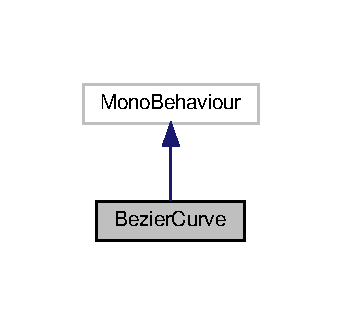
\includegraphics[width=164pt]{classBezierCurve__inherit__graph}
\end{center}
\end{figure}


Collaboration diagram for Bezier\+Curve\+:\nopagebreak
\begin{figure}[H]
\begin{center}
\leavevmode
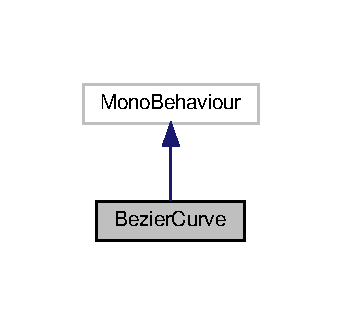
\includegraphics[width=164pt]{classBezierCurve__coll__graph}
\end{center}
\end{figure}
\subsection*{Public Member Functions}
\begin{DoxyCompactItemize}
\item 
Vector3 \hyperlink{classBezierCurve_a0ac697a04b35213e11d9c93a183ee7fe}{Get\+Point} (float t)
\item 
Vector3 \hyperlink{classBezierCurve_a3b39e1db5e230d6c4a89ec0386779efa}{Get\+Velocity} (float t)
\item 
void \hyperlink{classBezierCurve_a75b57f3aa46a6bb6679dfa79262e29ad}{Reset} ()
\item 
Vector3 \hyperlink{classBezierCurve_aee84a49317214403c6f59c2a60903662}{Get\+Direction} (float t)
\end{DoxyCompactItemize}
\subsection*{Public Attributes}
\begin{DoxyCompactItemize}
\item 
Vector3 \mbox{[}$\,$\mbox{]} \hyperlink{classBezierCurve_a77f62121b4b7ffb30b169d91691ebcbf}{points}
\end{DoxyCompactItemize}


\subsection{Member Function Documentation}
\mbox{\Hypertarget{classBezierCurve_aee84a49317214403c6f59c2a60903662}\label{classBezierCurve_aee84a49317214403c6f59c2a60903662}} 
\index{Bezier\+Curve@{Bezier\+Curve}!Get\+Direction@{Get\+Direction}}
\index{Get\+Direction@{Get\+Direction}!Bezier\+Curve@{Bezier\+Curve}}
\subsubsection{\texorpdfstring{Get\+Direction()}{GetDirection()}}
{\footnotesize\ttfamily Vector3 Bezier\+Curve.\+Get\+Direction (\begin{DoxyParamCaption}\item[{float}]{t }\end{DoxyParamCaption})\hspace{0.3cm}{\ttfamily [inline]}}

\mbox{\Hypertarget{classBezierCurve_a0ac697a04b35213e11d9c93a183ee7fe}\label{classBezierCurve_a0ac697a04b35213e11d9c93a183ee7fe}} 
\index{Bezier\+Curve@{Bezier\+Curve}!Get\+Point@{Get\+Point}}
\index{Get\+Point@{Get\+Point}!Bezier\+Curve@{Bezier\+Curve}}
\subsubsection{\texorpdfstring{Get\+Point()}{GetPoint()}}
{\footnotesize\ttfamily Vector3 Bezier\+Curve.\+Get\+Point (\begin{DoxyParamCaption}\item[{float}]{t }\end{DoxyParamCaption})\hspace{0.3cm}{\ttfamily [inline]}}

\mbox{\Hypertarget{classBezierCurve_a3b39e1db5e230d6c4a89ec0386779efa}\label{classBezierCurve_a3b39e1db5e230d6c4a89ec0386779efa}} 
\index{Bezier\+Curve@{Bezier\+Curve}!Get\+Velocity@{Get\+Velocity}}
\index{Get\+Velocity@{Get\+Velocity}!Bezier\+Curve@{Bezier\+Curve}}
\subsubsection{\texorpdfstring{Get\+Velocity()}{GetVelocity()}}
{\footnotesize\ttfamily Vector3 Bezier\+Curve.\+Get\+Velocity (\begin{DoxyParamCaption}\item[{float}]{t }\end{DoxyParamCaption})\hspace{0.3cm}{\ttfamily [inline]}}

\mbox{\Hypertarget{classBezierCurve_a75b57f3aa46a6bb6679dfa79262e29ad}\label{classBezierCurve_a75b57f3aa46a6bb6679dfa79262e29ad}} 
\index{Bezier\+Curve@{Bezier\+Curve}!Reset@{Reset}}
\index{Reset@{Reset}!Bezier\+Curve@{Bezier\+Curve}}
\subsubsection{\texorpdfstring{Reset()}{Reset()}}
{\footnotesize\ttfamily void Bezier\+Curve.\+Reset (\begin{DoxyParamCaption}{ }\end{DoxyParamCaption})\hspace{0.3cm}{\ttfamily [inline]}}



\subsection{Member Data Documentation}
\mbox{\Hypertarget{classBezierCurve_a77f62121b4b7ffb30b169d91691ebcbf}\label{classBezierCurve_a77f62121b4b7ffb30b169d91691ebcbf}} 
\index{Bezier\+Curve@{Bezier\+Curve}!points@{points}}
\index{points@{points}!Bezier\+Curve@{Bezier\+Curve}}
\subsubsection{\texorpdfstring{points}{points}}
{\footnotesize\ttfamily Vector3 \mbox{[}$\,$\mbox{]} Bezier\+Curve.\+points}



The documentation for this class was generated from the following file\+:\begin{DoxyCompactItemize}
\item 
/root/\+Documents/\+Unity\+\_\+\+S\+T40/\+Suratram\+\_\+mixed\+Reality\+Simulator/\+Assets/\+Scripts/\+Bezier/\hyperlink{BezierCurve_8cs}{Bezier\+Curve.\+cs}\end{DoxyCompactItemize}

\hypertarget{classBezierCurveInspector}{}\section{Bezier\+Curve\+Inspector Class Reference}
\label{classBezierCurveInspector}\index{Bezier\+Curve\+Inspector@{Bezier\+Curve\+Inspector}}


Inheritance diagram for Bezier\+Curve\+Inspector\+:\nopagebreak
\begin{figure}[H]
\begin{center}
\leavevmode
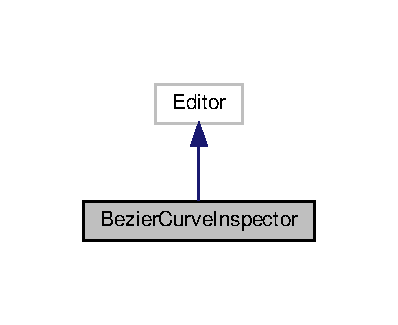
\includegraphics[width=191pt]{classBezierCurveInspector__inherit__graph}
\end{center}
\end{figure}


Collaboration diagram for Bezier\+Curve\+Inspector\+:\nopagebreak
\begin{figure}[H]
\begin{center}
\leavevmode
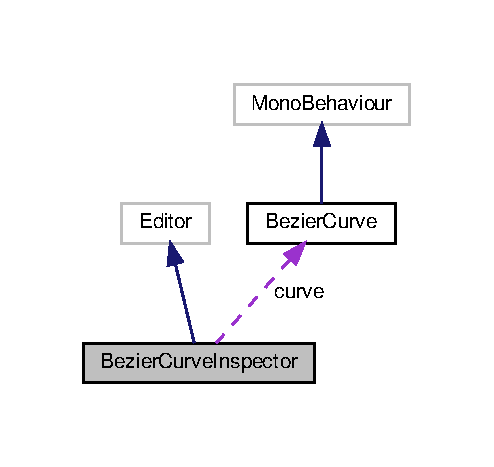
\includegraphics[width=237pt]{classBezierCurveInspector__coll__graph}
\end{center}
\end{figure}
\subsection*{Private Member Functions}
\begin{DoxyCompactItemize}
\item 
void \hyperlink{classBezierCurveInspector_abe87f2d75f12adc52633e1d9ba483e32}{On\+Scene\+G\+UI} ()
\item 
void \hyperlink{classBezierCurveInspector_a586dff51b6f0a328f1d4df96fb4bcea6}{Show\+Directions} ()
\item 
Vector3 \hyperlink{classBezierCurveInspector_aa9ed65ee21a6d05f6ed51760fc5d4c08}{Show\+Point} (int index)
\end{DoxyCompactItemize}
\subsection*{Private Attributes}
\begin{DoxyCompactItemize}
\item 
const int \hyperlink{classBezierCurveInspector_a6bc9700906d0eb59f3a6ef077babce50}{line\+Steps} = 10
\item 
\hyperlink{classBezierCurve}{Bezier\+Curve} \hyperlink{classBezierCurveInspector_a8e0c756972b42dd58803eb055552a8d9}{curve}
\item 
Transform \hyperlink{classBezierCurveInspector_a556d6234e17e3c8edefb2a2558fd4fe6}{handle\+Transform}
\item 
Quaternion \hyperlink{classBezierCurveInspector_aaec6692f6b6048be6186b642ca783df4}{handle\+Rotation}
\item 
const float \hyperlink{classBezierCurveInspector_ad1b331e90f079da9c65c12387db2ad6d}{direction\+Scale} = 0.\+5f
\end{DoxyCompactItemize}


\subsection{Member Function Documentation}
\mbox{\Hypertarget{classBezierCurveInspector_abe87f2d75f12adc52633e1d9ba483e32}\label{classBezierCurveInspector_abe87f2d75f12adc52633e1d9ba483e32}} 
\index{Bezier\+Curve\+Inspector@{Bezier\+Curve\+Inspector}!On\+Scene\+G\+UI@{On\+Scene\+G\+UI}}
\index{On\+Scene\+G\+UI@{On\+Scene\+G\+UI}!Bezier\+Curve\+Inspector@{Bezier\+Curve\+Inspector}}
\subsubsection{\texorpdfstring{On\+Scene\+G\+U\+I()}{OnSceneGUI()}}
{\footnotesize\ttfamily void Bezier\+Curve\+Inspector.\+On\+Scene\+G\+UI (\begin{DoxyParamCaption}{ }\end{DoxyParamCaption})\hspace{0.3cm}{\ttfamily [inline]}, {\ttfamily [private]}}

\mbox{\Hypertarget{classBezierCurveInspector_a586dff51b6f0a328f1d4df96fb4bcea6}\label{classBezierCurveInspector_a586dff51b6f0a328f1d4df96fb4bcea6}} 
\index{Bezier\+Curve\+Inspector@{Bezier\+Curve\+Inspector}!Show\+Directions@{Show\+Directions}}
\index{Show\+Directions@{Show\+Directions}!Bezier\+Curve\+Inspector@{Bezier\+Curve\+Inspector}}
\subsubsection{\texorpdfstring{Show\+Directions()}{ShowDirections()}}
{\footnotesize\ttfamily void Bezier\+Curve\+Inspector.\+Show\+Directions (\begin{DoxyParamCaption}{ }\end{DoxyParamCaption})\hspace{0.3cm}{\ttfamily [inline]}, {\ttfamily [private]}}

\mbox{\Hypertarget{classBezierCurveInspector_aa9ed65ee21a6d05f6ed51760fc5d4c08}\label{classBezierCurveInspector_aa9ed65ee21a6d05f6ed51760fc5d4c08}} 
\index{Bezier\+Curve\+Inspector@{Bezier\+Curve\+Inspector}!Show\+Point@{Show\+Point}}
\index{Show\+Point@{Show\+Point}!Bezier\+Curve\+Inspector@{Bezier\+Curve\+Inspector}}
\subsubsection{\texorpdfstring{Show\+Point()}{ShowPoint()}}
{\footnotesize\ttfamily Vector3 Bezier\+Curve\+Inspector.\+Show\+Point (\begin{DoxyParamCaption}\item[{int}]{index }\end{DoxyParamCaption})\hspace{0.3cm}{\ttfamily [inline]}, {\ttfamily [private]}}



\subsection{Member Data Documentation}
\mbox{\Hypertarget{classBezierCurveInspector_a8e0c756972b42dd58803eb055552a8d9}\label{classBezierCurveInspector_a8e0c756972b42dd58803eb055552a8d9}} 
\index{Bezier\+Curve\+Inspector@{Bezier\+Curve\+Inspector}!curve@{curve}}
\index{curve@{curve}!Bezier\+Curve\+Inspector@{Bezier\+Curve\+Inspector}}
\subsubsection{\texorpdfstring{curve}{curve}}
{\footnotesize\ttfamily \hyperlink{classBezierCurve}{Bezier\+Curve} Bezier\+Curve\+Inspector.\+curve\hspace{0.3cm}{\ttfamily [private]}}

\mbox{\Hypertarget{classBezierCurveInspector_ad1b331e90f079da9c65c12387db2ad6d}\label{classBezierCurveInspector_ad1b331e90f079da9c65c12387db2ad6d}} 
\index{Bezier\+Curve\+Inspector@{Bezier\+Curve\+Inspector}!direction\+Scale@{direction\+Scale}}
\index{direction\+Scale@{direction\+Scale}!Bezier\+Curve\+Inspector@{Bezier\+Curve\+Inspector}}
\subsubsection{\texorpdfstring{direction\+Scale}{directionScale}}
{\footnotesize\ttfamily const float Bezier\+Curve\+Inspector.\+direction\+Scale = 0.\+5f\hspace{0.3cm}{\ttfamily [private]}}

\mbox{\Hypertarget{classBezierCurveInspector_aaec6692f6b6048be6186b642ca783df4}\label{classBezierCurveInspector_aaec6692f6b6048be6186b642ca783df4}} 
\index{Bezier\+Curve\+Inspector@{Bezier\+Curve\+Inspector}!handle\+Rotation@{handle\+Rotation}}
\index{handle\+Rotation@{handle\+Rotation}!Bezier\+Curve\+Inspector@{Bezier\+Curve\+Inspector}}
\subsubsection{\texorpdfstring{handle\+Rotation}{handleRotation}}
{\footnotesize\ttfamily Quaternion Bezier\+Curve\+Inspector.\+handle\+Rotation\hspace{0.3cm}{\ttfamily [private]}}

\mbox{\Hypertarget{classBezierCurveInspector_a556d6234e17e3c8edefb2a2558fd4fe6}\label{classBezierCurveInspector_a556d6234e17e3c8edefb2a2558fd4fe6}} 
\index{Bezier\+Curve\+Inspector@{Bezier\+Curve\+Inspector}!handle\+Transform@{handle\+Transform}}
\index{handle\+Transform@{handle\+Transform}!Bezier\+Curve\+Inspector@{Bezier\+Curve\+Inspector}}
\subsubsection{\texorpdfstring{handle\+Transform}{handleTransform}}
{\footnotesize\ttfamily Transform Bezier\+Curve\+Inspector.\+handle\+Transform\hspace{0.3cm}{\ttfamily [private]}}

\mbox{\Hypertarget{classBezierCurveInspector_a6bc9700906d0eb59f3a6ef077babce50}\label{classBezierCurveInspector_a6bc9700906d0eb59f3a6ef077babce50}} 
\index{Bezier\+Curve\+Inspector@{Bezier\+Curve\+Inspector}!line\+Steps@{line\+Steps}}
\index{line\+Steps@{line\+Steps}!Bezier\+Curve\+Inspector@{Bezier\+Curve\+Inspector}}
\subsubsection{\texorpdfstring{line\+Steps}{lineSteps}}
{\footnotesize\ttfamily const int Bezier\+Curve\+Inspector.\+line\+Steps = 10\hspace{0.3cm}{\ttfamily [private]}}



The documentation for this class was generated from the following file\+:\begin{DoxyCompactItemize}
\item 
/root/\+Documents/\+Unity\+\_\+\+S\+T40/\+Suratram\+\_\+mixed\+Reality\+Simulator/\+Assets/\+Scripts/\+Bezier/\+Editor/\hyperlink{BezierCurveInspector_8cs}{Bezier\+Curve\+Inspector.\+cs}\end{DoxyCompactItemize}

\hypertarget{classBezierSpline}{}\section{Bezier\+Spline Class Reference}
\label{classBezierSpline}\index{Bezier\+Spline@{Bezier\+Spline}}


Inheritance diagram for Bezier\+Spline\+:\nopagebreak
\begin{figure}[H]
\begin{center}
\leavevmode
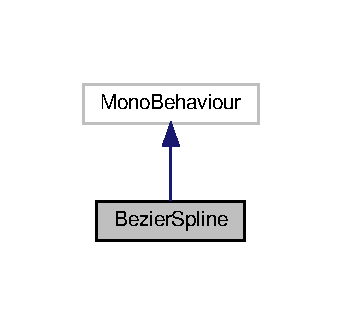
\includegraphics[width=164pt]{classBezierSpline__inherit__graph}
\end{center}
\end{figure}


Collaboration diagram for Bezier\+Spline\+:\nopagebreak
\begin{figure}[H]
\begin{center}
\leavevmode
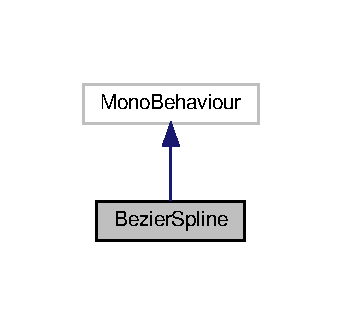
\includegraphics[width=164pt]{classBezierSpline__coll__graph}
\end{center}
\end{figure}
\subsection*{Public Member Functions}
\begin{DoxyCompactItemize}
\item 
Vector3 \hyperlink{classBezierSpline_a4a9993e2dafa4a6b8819d94a25c70245}{Get\+Point} (float t)
\item 
Vector3 \hyperlink{classBezierSpline_a0d8c73af995773501fd3e5c4dac4c3b6}{Get\+Velocity} (float t)
\item 
Vector3 \hyperlink{classBezierSpline_a24c9b2087b16b650871a9ed2355987cc}{Get\+Direction} (float t)
\item 
void \hyperlink{classBezierSpline_a4676e1c6d2cfc8454c028e30d54783bd}{Add\+Curve} ()
\item 
void \hyperlink{classBezierSpline_a69c0d6f430f28fec72bffb8812861247}{Reset} ()
\item 
Vector3 \hyperlink{classBezierSpline_aee83e5e470e3d7d23f75875c81bbd326}{Get\+Control\+Point} (int index)
\item 
void \hyperlink{classBezierSpline_aed423df0d5f7c31a82a617ad8ebc23e4}{Set\+Control\+Point} (int index, Vector3 point)
\item 
\hyperlink{BezierControlPointMode_8cs_a41ff1a7271616f36cab397d937ee41b0}{Bezier\+Control\+Point\+Mode} \hyperlink{classBezierSpline_a1600b5bf35f1aa796e5fbe227b5a767d}{Get\+Control\+Point\+Mode} (int index)
\item 
void \hyperlink{classBezierSpline_a5c538c5216c5743de35ce9999760749c}{Set\+Control\+Point\+Mode} (int index, \hyperlink{BezierControlPointMode_8cs_a41ff1a7271616f36cab397d937ee41b0}{Bezier\+Control\+Point\+Mode} mode)
\end{DoxyCompactItemize}
\subsection*{Properties}
\begin{DoxyCompactItemize}
\item 
bool \hyperlink{classBezierSpline_a9b13fb8edeb86c6166fbd091b044eb63}{Loop}\hspace{0.3cm}{\ttfamily  \mbox{[}get, set\mbox{]}}
\item 
int \hyperlink{classBezierSpline_a953275346ac1b490473e3500c06b6286}{Curve\+Count}\hspace{0.3cm}{\ttfamily  \mbox{[}get\mbox{]}}
\item 
int \hyperlink{classBezierSpline_acb5b34c12c98bdf6b0ec0917009b1626}{Control\+Point\+Count}\hspace{0.3cm}{\ttfamily  \mbox{[}get\mbox{]}}
\end{DoxyCompactItemize}
\subsection*{Private Member Functions}
\begin{DoxyCompactItemize}
\item 
void \hyperlink{classBezierSpline_a9ce5f77aeb9b671034ce0845f8539166}{Enforce\+Mode} (int index)
\end{DoxyCompactItemize}
\subsection*{Private Attributes}
\begin{DoxyCompactItemize}
\item 
Vector3 \mbox{[}$\,$\mbox{]} \hyperlink{classBezierSpline_adda54d62157465856c511f0b94fd78d9}{points}
\item 
\hyperlink{BezierControlPointMode_8cs_a41ff1a7271616f36cab397d937ee41b0}{Bezier\+Control\+Point\+Mode} \mbox{[}$\,$\mbox{]} \hyperlink{classBezierSpline_affe3fe5b3977dfedf13f40e433363010}{modes}
\item 
bool \hyperlink{classBezierSpline_a819d3c15ebc913ed8da39daa07fd89a7}{loop}
\end{DoxyCompactItemize}


\subsection{Member Function Documentation}
\mbox{\Hypertarget{classBezierSpline_a4676e1c6d2cfc8454c028e30d54783bd}\label{classBezierSpline_a4676e1c6d2cfc8454c028e30d54783bd}} 
\index{Bezier\+Spline@{Bezier\+Spline}!Add\+Curve@{Add\+Curve}}
\index{Add\+Curve@{Add\+Curve}!Bezier\+Spline@{Bezier\+Spline}}
\subsubsection{\texorpdfstring{Add\+Curve()}{AddCurve()}}
{\footnotesize\ttfamily void Bezier\+Spline.\+Add\+Curve (\begin{DoxyParamCaption}{ }\end{DoxyParamCaption})\hspace{0.3cm}{\ttfamily [inline]}}

\mbox{\Hypertarget{classBezierSpline_a9ce5f77aeb9b671034ce0845f8539166}\label{classBezierSpline_a9ce5f77aeb9b671034ce0845f8539166}} 
\index{Bezier\+Spline@{Bezier\+Spline}!Enforce\+Mode@{Enforce\+Mode}}
\index{Enforce\+Mode@{Enforce\+Mode}!Bezier\+Spline@{Bezier\+Spline}}
\subsubsection{\texorpdfstring{Enforce\+Mode()}{EnforceMode()}}
{\footnotesize\ttfamily void Bezier\+Spline.\+Enforce\+Mode (\begin{DoxyParamCaption}\item[{int}]{index }\end{DoxyParamCaption})\hspace{0.3cm}{\ttfamily [inline]}, {\ttfamily [private]}}

\mbox{\Hypertarget{classBezierSpline_aee83e5e470e3d7d23f75875c81bbd326}\label{classBezierSpline_aee83e5e470e3d7d23f75875c81bbd326}} 
\index{Bezier\+Spline@{Bezier\+Spline}!Get\+Control\+Point@{Get\+Control\+Point}}
\index{Get\+Control\+Point@{Get\+Control\+Point}!Bezier\+Spline@{Bezier\+Spline}}
\subsubsection{\texorpdfstring{Get\+Control\+Point()}{GetControlPoint()}}
{\footnotesize\ttfamily Vector3 Bezier\+Spline.\+Get\+Control\+Point (\begin{DoxyParamCaption}\item[{int}]{index }\end{DoxyParamCaption})\hspace{0.3cm}{\ttfamily [inline]}}

\mbox{\Hypertarget{classBezierSpline_a1600b5bf35f1aa796e5fbe227b5a767d}\label{classBezierSpline_a1600b5bf35f1aa796e5fbe227b5a767d}} 
\index{Bezier\+Spline@{Bezier\+Spline}!Get\+Control\+Point\+Mode@{Get\+Control\+Point\+Mode}}
\index{Get\+Control\+Point\+Mode@{Get\+Control\+Point\+Mode}!Bezier\+Spline@{Bezier\+Spline}}
\subsubsection{\texorpdfstring{Get\+Control\+Point\+Mode()}{GetControlPointMode()}}
{\footnotesize\ttfamily \hyperlink{BezierControlPointMode_8cs_a41ff1a7271616f36cab397d937ee41b0}{Bezier\+Control\+Point\+Mode} Bezier\+Spline.\+Get\+Control\+Point\+Mode (\begin{DoxyParamCaption}\item[{int}]{index }\end{DoxyParamCaption})\hspace{0.3cm}{\ttfamily [inline]}}

\mbox{\Hypertarget{classBezierSpline_a24c9b2087b16b650871a9ed2355987cc}\label{classBezierSpline_a24c9b2087b16b650871a9ed2355987cc}} 
\index{Bezier\+Spline@{Bezier\+Spline}!Get\+Direction@{Get\+Direction}}
\index{Get\+Direction@{Get\+Direction}!Bezier\+Spline@{Bezier\+Spline}}
\subsubsection{\texorpdfstring{Get\+Direction()}{GetDirection()}}
{\footnotesize\ttfamily Vector3 Bezier\+Spline.\+Get\+Direction (\begin{DoxyParamCaption}\item[{float}]{t }\end{DoxyParamCaption})\hspace{0.3cm}{\ttfamily [inline]}}

\mbox{\Hypertarget{classBezierSpline_a4a9993e2dafa4a6b8819d94a25c70245}\label{classBezierSpline_a4a9993e2dafa4a6b8819d94a25c70245}} 
\index{Bezier\+Spline@{Bezier\+Spline}!Get\+Point@{Get\+Point}}
\index{Get\+Point@{Get\+Point}!Bezier\+Spline@{Bezier\+Spline}}
\subsubsection{\texorpdfstring{Get\+Point()}{GetPoint()}}
{\footnotesize\ttfamily Vector3 Bezier\+Spline.\+Get\+Point (\begin{DoxyParamCaption}\item[{float}]{t }\end{DoxyParamCaption})\hspace{0.3cm}{\ttfamily [inline]}}

\mbox{\Hypertarget{classBezierSpline_a0d8c73af995773501fd3e5c4dac4c3b6}\label{classBezierSpline_a0d8c73af995773501fd3e5c4dac4c3b6}} 
\index{Bezier\+Spline@{Bezier\+Spline}!Get\+Velocity@{Get\+Velocity}}
\index{Get\+Velocity@{Get\+Velocity}!Bezier\+Spline@{Bezier\+Spline}}
\subsubsection{\texorpdfstring{Get\+Velocity()}{GetVelocity()}}
{\footnotesize\ttfamily Vector3 Bezier\+Spline.\+Get\+Velocity (\begin{DoxyParamCaption}\item[{float}]{t }\end{DoxyParamCaption})\hspace{0.3cm}{\ttfamily [inline]}}

\mbox{\Hypertarget{classBezierSpline_a69c0d6f430f28fec72bffb8812861247}\label{classBezierSpline_a69c0d6f430f28fec72bffb8812861247}} 
\index{Bezier\+Spline@{Bezier\+Spline}!Reset@{Reset}}
\index{Reset@{Reset}!Bezier\+Spline@{Bezier\+Spline}}
\subsubsection{\texorpdfstring{Reset()}{Reset()}}
{\footnotesize\ttfamily void Bezier\+Spline.\+Reset (\begin{DoxyParamCaption}{ }\end{DoxyParamCaption})\hspace{0.3cm}{\ttfamily [inline]}}

\mbox{\Hypertarget{classBezierSpline_aed423df0d5f7c31a82a617ad8ebc23e4}\label{classBezierSpline_aed423df0d5f7c31a82a617ad8ebc23e4}} 
\index{Bezier\+Spline@{Bezier\+Spline}!Set\+Control\+Point@{Set\+Control\+Point}}
\index{Set\+Control\+Point@{Set\+Control\+Point}!Bezier\+Spline@{Bezier\+Spline}}
\subsubsection{\texorpdfstring{Set\+Control\+Point()}{SetControlPoint()}}
{\footnotesize\ttfamily void Bezier\+Spline.\+Set\+Control\+Point (\begin{DoxyParamCaption}\item[{int}]{index,  }\item[{Vector3}]{point }\end{DoxyParamCaption})\hspace{0.3cm}{\ttfamily [inline]}}

\mbox{\Hypertarget{classBezierSpline_a5c538c5216c5743de35ce9999760749c}\label{classBezierSpline_a5c538c5216c5743de35ce9999760749c}} 
\index{Bezier\+Spline@{Bezier\+Spline}!Set\+Control\+Point\+Mode@{Set\+Control\+Point\+Mode}}
\index{Set\+Control\+Point\+Mode@{Set\+Control\+Point\+Mode}!Bezier\+Spline@{Bezier\+Spline}}
\subsubsection{\texorpdfstring{Set\+Control\+Point\+Mode()}{SetControlPointMode()}}
{\footnotesize\ttfamily void Bezier\+Spline.\+Set\+Control\+Point\+Mode (\begin{DoxyParamCaption}\item[{int}]{index,  }\item[{\hyperlink{BezierControlPointMode_8cs_a41ff1a7271616f36cab397d937ee41b0}{Bezier\+Control\+Point\+Mode}}]{mode }\end{DoxyParamCaption})\hspace{0.3cm}{\ttfamily [inline]}}



\subsection{Member Data Documentation}
\mbox{\Hypertarget{classBezierSpline_a819d3c15ebc913ed8da39daa07fd89a7}\label{classBezierSpline_a819d3c15ebc913ed8da39daa07fd89a7}} 
\index{Bezier\+Spline@{Bezier\+Spline}!loop@{loop}}
\index{loop@{loop}!Bezier\+Spline@{Bezier\+Spline}}
\subsubsection{\texorpdfstring{loop}{loop}}
{\footnotesize\ttfamily bool Bezier\+Spline.\+loop\hspace{0.3cm}{\ttfamily [private]}}

\mbox{\Hypertarget{classBezierSpline_affe3fe5b3977dfedf13f40e433363010}\label{classBezierSpline_affe3fe5b3977dfedf13f40e433363010}} 
\index{Bezier\+Spline@{Bezier\+Spline}!modes@{modes}}
\index{modes@{modes}!Bezier\+Spline@{Bezier\+Spline}}
\subsubsection{\texorpdfstring{modes}{modes}}
{\footnotesize\ttfamily \hyperlink{BezierControlPointMode_8cs_a41ff1a7271616f36cab397d937ee41b0}{Bezier\+Control\+Point\+Mode} \mbox{[}$\,$\mbox{]} Bezier\+Spline.\+modes\hspace{0.3cm}{\ttfamily [private]}}

\mbox{\Hypertarget{classBezierSpline_adda54d62157465856c511f0b94fd78d9}\label{classBezierSpline_adda54d62157465856c511f0b94fd78d9}} 
\index{Bezier\+Spline@{Bezier\+Spline}!points@{points}}
\index{points@{points}!Bezier\+Spline@{Bezier\+Spline}}
\subsubsection{\texorpdfstring{points}{points}}
{\footnotesize\ttfamily Vector3 \mbox{[}$\,$\mbox{]} Bezier\+Spline.\+points\hspace{0.3cm}{\ttfamily [private]}}



\subsection{Property Documentation}
\mbox{\Hypertarget{classBezierSpline_acb5b34c12c98bdf6b0ec0917009b1626}\label{classBezierSpline_acb5b34c12c98bdf6b0ec0917009b1626}} 
\index{Bezier\+Spline@{Bezier\+Spline}!Control\+Point\+Count@{Control\+Point\+Count}}
\index{Control\+Point\+Count@{Control\+Point\+Count}!Bezier\+Spline@{Bezier\+Spline}}
\subsubsection{\texorpdfstring{Control\+Point\+Count}{ControlPointCount}}
{\footnotesize\ttfamily int Bezier\+Spline.\+Control\+Point\+Count\hspace{0.3cm}{\ttfamily [get]}}

\mbox{\Hypertarget{classBezierSpline_a953275346ac1b490473e3500c06b6286}\label{classBezierSpline_a953275346ac1b490473e3500c06b6286}} 
\index{Bezier\+Spline@{Bezier\+Spline}!Curve\+Count@{Curve\+Count}}
\index{Curve\+Count@{Curve\+Count}!Bezier\+Spline@{Bezier\+Spline}}
\subsubsection{\texorpdfstring{Curve\+Count}{CurveCount}}
{\footnotesize\ttfamily int Bezier\+Spline.\+Curve\+Count\hspace{0.3cm}{\ttfamily [get]}}

\mbox{\Hypertarget{classBezierSpline_a9b13fb8edeb86c6166fbd091b044eb63}\label{classBezierSpline_a9b13fb8edeb86c6166fbd091b044eb63}} 
\index{Bezier\+Spline@{Bezier\+Spline}!Loop@{Loop}}
\index{Loop@{Loop}!Bezier\+Spline@{Bezier\+Spline}}
\subsubsection{\texorpdfstring{Loop}{Loop}}
{\footnotesize\ttfamily bool Bezier\+Spline.\+Loop\hspace{0.3cm}{\ttfamily [get]}, {\ttfamily [set]}}



The documentation for this class was generated from the following file\+:\begin{DoxyCompactItemize}
\item 
/root/\+Documents/\+Unity\+\_\+\+S\+T40/\+Suratram\+\_\+mixed\+Reality\+Simulator/\+Assets/\+Scripts/\+Bezier/\hyperlink{BezierSpline_8cs}{Bezier\+Spline.\+cs}\end{DoxyCompactItemize}

\hypertarget{classBezierSplineInspector}{}\section{Bezier\+Spline\+Inspector Class Reference}
\label{classBezierSplineInspector}\index{Bezier\+Spline\+Inspector@{Bezier\+Spline\+Inspector}}


Inheritance diagram for Bezier\+Spline\+Inspector\+:\nopagebreak
\begin{figure}[H]
\begin{center}
\leavevmode
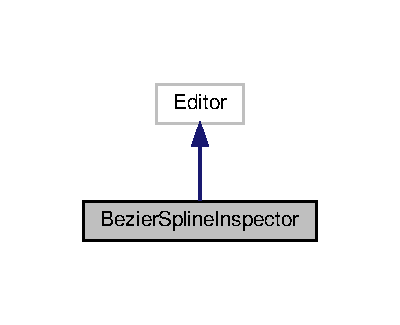
\includegraphics[width=192pt]{classBezierSplineInspector__inherit__graph}
\end{center}
\end{figure}


Collaboration diagram for Bezier\+Spline\+Inspector\+:\nopagebreak
\begin{figure}[H]
\begin{center}
\leavevmode
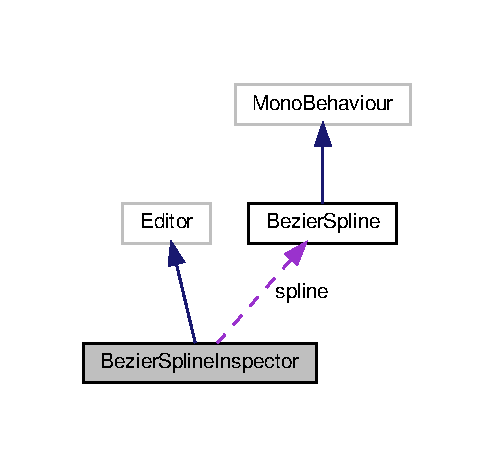
\includegraphics[width=237pt]{classBezierSplineInspector__coll__graph}
\end{center}
\end{figure}
\subsection*{Public Member Functions}
\begin{DoxyCompactItemize}
\item 
override void \hyperlink{classBezierSplineInspector_a3232a5fd28ba98bf7b5d4aa170546f31}{On\+Inspector\+G\+UI} ()
\end{DoxyCompactItemize}
\subsection*{Private Member Functions}
\begin{DoxyCompactItemize}
\item 
void \hyperlink{classBezierSplineInspector_a1b5db10b5a3a743cbd2895cc61faad23}{On\+Scene\+G\+UI} ()
\item 
Vector3 \hyperlink{classBezierSplineInspector_a413aaf08e6210a0613ec05ee97ca93dc}{Show\+Point} (int index)
\item 
void \hyperlink{classBezierSplineInspector_a1fab28bf9747a0e23dcae459f9d965b7}{Show\+Directions} ()
\item 
void \hyperlink{classBezierSplineInspector_a9301f0b079b6a96ff147231bb6af0bfe}{Draw\+Selected\+Point\+Inspector} ()
\end{DoxyCompactItemize}
\subsection*{Private Attributes}
\begin{DoxyCompactItemize}
\item 
const int \hyperlink{classBezierSplineInspector_a6cc82c82cb437fc3a75a5b2b8f6d5789}{line\+Steps} = 10
\item 
const float \hyperlink{classBezierSplineInspector_a574e20490bad6dbaf9024fa6cc6d4d24}{direction\+Scale} = 0.\+5f
\item 
const int \hyperlink{classBezierSplineInspector_a444eba3ff5695e7b87c042ad7e2ee0aa}{steps\+Per\+Curve} = 10
\item 
const float \hyperlink{classBezierSplineInspector_ac9749fa64c910242d064f1a6c924fa98}{handle\+Size} = 0.\+04f
\item 
const float \hyperlink{classBezierSplineInspector_acc93b6778c8674ec2b57d48a1466bcd6}{pick\+Size} = 0.\+06f
\item 
int \hyperlink{classBezierSplineInspector_af0b7882ca31e32db00b624a622f001d1}{selected\+Index} = -\/1
\item 
\hyperlink{classBezierSpline}{Bezier\+Spline} \hyperlink{classBezierSplineInspector_a13f1a0472f67bdf873d1e34d2ed5ff32}{spline}
\item 
Transform \hyperlink{classBezierSplineInspector_a735dfdff25b8fd3ea904c73584648667}{handle\+Transform}
\item 
Quaternion \hyperlink{classBezierSplineInspector_a6ba4d222ada9cfeeb4f36e2649c4f286}{handle\+Rotation}
\end{DoxyCompactItemize}
\subsection*{Static Private Attributes}
\begin{DoxyCompactItemize}
\item 
static Color \mbox{[}$\,$\mbox{]} \hyperlink{classBezierSplineInspector_a20cbc0fdf235b0b9e2d349def79ba333}{mode\+Colors}
\end{DoxyCompactItemize}


\subsection{Member Function Documentation}
\mbox{\Hypertarget{classBezierSplineInspector_a9301f0b079b6a96ff147231bb6af0bfe}\label{classBezierSplineInspector_a9301f0b079b6a96ff147231bb6af0bfe}} 
\index{Bezier\+Spline\+Inspector@{Bezier\+Spline\+Inspector}!Draw\+Selected\+Point\+Inspector@{Draw\+Selected\+Point\+Inspector}}
\index{Draw\+Selected\+Point\+Inspector@{Draw\+Selected\+Point\+Inspector}!Bezier\+Spline\+Inspector@{Bezier\+Spline\+Inspector}}
\subsubsection{\texorpdfstring{Draw\+Selected\+Point\+Inspector()}{DrawSelectedPointInspector()}}
{\footnotesize\ttfamily void Bezier\+Spline\+Inspector.\+Draw\+Selected\+Point\+Inspector (\begin{DoxyParamCaption}{ }\end{DoxyParamCaption})\hspace{0.3cm}{\ttfamily [inline]}, {\ttfamily [private]}}

\mbox{\Hypertarget{classBezierSplineInspector_a3232a5fd28ba98bf7b5d4aa170546f31}\label{classBezierSplineInspector_a3232a5fd28ba98bf7b5d4aa170546f31}} 
\index{Bezier\+Spline\+Inspector@{Bezier\+Spline\+Inspector}!On\+Inspector\+G\+UI@{On\+Inspector\+G\+UI}}
\index{On\+Inspector\+G\+UI@{On\+Inspector\+G\+UI}!Bezier\+Spline\+Inspector@{Bezier\+Spline\+Inspector}}
\subsubsection{\texorpdfstring{On\+Inspector\+G\+U\+I()}{OnInspectorGUI()}}
{\footnotesize\ttfamily override void Bezier\+Spline\+Inspector.\+On\+Inspector\+G\+UI (\begin{DoxyParamCaption}{ }\end{DoxyParamCaption})\hspace{0.3cm}{\ttfamily [inline]}}

\mbox{\Hypertarget{classBezierSplineInspector_a1b5db10b5a3a743cbd2895cc61faad23}\label{classBezierSplineInspector_a1b5db10b5a3a743cbd2895cc61faad23}} 
\index{Bezier\+Spline\+Inspector@{Bezier\+Spline\+Inspector}!On\+Scene\+G\+UI@{On\+Scene\+G\+UI}}
\index{On\+Scene\+G\+UI@{On\+Scene\+G\+UI}!Bezier\+Spline\+Inspector@{Bezier\+Spline\+Inspector}}
\subsubsection{\texorpdfstring{On\+Scene\+G\+U\+I()}{OnSceneGUI()}}
{\footnotesize\ttfamily void Bezier\+Spline\+Inspector.\+On\+Scene\+G\+UI (\begin{DoxyParamCaption}{ }\end{DoxyParamCaption})\hspace{0.3cm}{\ttfamily [inline]}, {\ttfamily [private]}}

\mbox{\Hypertarget{classBezierSplineInspector_a1fab28bf9747a0e23dcae459f9d965b7}\label{classBezierSplineInspector_a1fab28bf9747a0e23dcae459f9d965b7}} 
\index{Bezier\+Spline\+Inspector@{Bezier\+Spline\+Inspector}!Show\+Directions@{Show\+Directions}}
\index{Show\+Directions@{Show\+Directions}!Bezier\+Spline\+Inspector@{Bezier\+Spline\+Inspector}}
\subsubsection{\texorpdfstring{Show\+Directions()}{ShowDirections()}}
{\footnotesize\ttfamily void Bezier\+Spline\+Inspector.\+Show\+Directions (\begin{DoxyParamCaption}{ }\end{DoxyParamCaption})\hspace{0.3cm}{\ttfamily [inline]}, {\ttfamily [private]}}

\mbox{\Hypertarget{classBezierSplineInspector_a413aaf08e6210a0613ec05ee97ca93dc}\label{classBezierSplineInspector_a413aaf08e6210a0613ec05ee97ca93dc}} 
\index{Bezier\+Spline\+Inspector@{Bezier\+Spline\+Inspector}!Show\+Point@{Show\+Point}}
\index{Show\+Point@{Show\+Point}!Bezier\+Spline\+Inspector@{Bezier\+Spline\+Inspector}}
\subsubsection{\texorpdfstring{Show\+Point()}{ShowPoint()}}
{\footnotesize\ttfamily Vector3 Bezier\+Spline\+Inspector.\+Show\+Point (\begin{DoxyParamCaption}\item[{int}]{index }\end{DoxyParamCaption})\hspace{0.3cm}{\ttfamily [inline]}, {\ttfamily [private]}}



\subsection{Member Data Documentation}
\mbox{\Hypertarget{classBezierSplineInspector_a574e20490bad6dbaf9024fa6cc6d4d24}\label{classBezierSplineInspector_a574e20490bad6dbaf9024fa6cc6d4d24}} 
\index{Bezier\+Spline\+Inspector@{Bezier\+Spline\+Inspector}!direction\+Scale@{direction\+Scale}}
\index{direction\+Scale@{direction\+Scale}!Bezier\+Spline\+Inspector@{Bezier\+Spline\+Inspector}}
\subsubsection{\texorpdfstring{direction\+Scale}{directionScale}}
{\footnotesize\ttfamily const float Bezier\+Spline\+Inspector.\+direction\+Scale = 0.\+5f\hspace{0.3cm}{\ttfamily [private]}}

\mbox{\Hypertarget{classBezierSplineInspector_a6ba4d222ada9cfeeb4f36e2649c4f286}\label{classBezierSplineInspector_a6ba4d222ada9cfeeb4f36e2649c4f286}} 
\index{Bezier\+Spline\+Inspector@{Bezier\+Spline\+Inspector}!handle\+Rotation@{handle\+Rotation}}
\index{handle\+Rotation@{handle\+Rotation}!Bezier\+Spline\+Inspector@{Bezier\+Spline\+Inspector}}
\subsubsection{\texorpdfstring{handle\+Rotation}{handleRotation}}
{\footnotesize\ttfamily Quaternion Bezier\+Spline\+Inspector.\+handle\+Rotation\hspace{0.3cm}{\ttfamily [private]}}

\mbox{\Hypertarget{classBezierSplineInspector_ac9749fa64c910242d064f1a6c924fa98}\label{classBezierSplineInspector_ac9749fa64c910242d064f1a6c924fa98}} 
\index{Bezier\+Spline\+Inspector@{Bezier\+Spline\+Inspector}!handle\+Size@{handle\+Size}}
\index{handle\+Size@{handle\+Size}!Bezier\+Spline\+Inspector@{Bezier\+Spline\+Inspector}}
\subsubsection{\texorpdfstring{handle\+Size}{handleSize}}
{\footnotesize\ttfamily const float Bezier\+Spline\+Inspector.\+handle\+Size = 0.\+04f\hspace{0.3cm}{\ttfamily [private]}}

\mbox{\Hypertarget{classBezierSplineInspector_a735dfdff25b8fd3ea904c73584648667}\label{classBezierSplineInspector_a735dfdff25b8fd3ea904c73584648667}} 
\index{Bezier\+Spline\+Inspector@{Bezier\+Spline\+Inspector}!handle\+Transform@{handle\+Transform}}
\index{handle\+Transform@{handle\+Transform}!Bezier\+Spline\+Inspector@{Bezier\+Spline\+Inspector}}
\subsubsection{\texorpdfstring{handle\+Transform}{handleTransform}}
{\footnotesize\ttfamily Transform Bezier\+Spline\+Inspector.\+handle\+Transform\hspace{0.3cm}{\ttfamily [private]}}

\mbox{\Hypertarget{classBezierSplineInspector_a6cc82c82cb437fc3a75a5b2b8f6d5789}\label{classBezierSplineInspector_a6cc82c82cb437fc3a75a5b2b8f6d5789}} 
\index{Bezier\+Spline\+Inspector@{Bezier\+Spline\+Inspector}!line\+Steps@{line\+Steps}}
\index{line\+Steps@{line\+Steps}!Bezier\+Spline\+Inspector@{Bezier\+Spline\+Inspector}}
\subsubsection{\texorpdfstring{line\+Steps}{lineSteps}}
{\footnotesize\ttfamily const int Bezier\+Spline\+Inspector.\+line\+Steps = 10\hspace{0.3cm}{\ttfamily [private]}}

\mbox{\Hypertarget{classBezierSplineInspector_a20cbc0fdf235b0b9e2d349def79ba333}\label{classBezierSplineInspector_a20cbc0fdf235b0b9e2d349def79ba333}} 
\index{Bezier\+Spline\+Inspector@{Bezier\+Spline\+Inspector}!mode\+Colors@{mode\+Colors}}
\index{mode\+Colors@{mode\+Colors}!Bezier\+Spline\+Inspector@{Bezier\+Spline\+Inspector}}
\subsubsection{\texorpdfstring{mode\+Colors}{modeColors}}
{\footnotesize\ttfamily Color \mbox{[}$\,$\mbox{]} Bezier\+Spline\+Inspector.\+mode\+Colors\hspace{0.3cm}{\ttfamily [static]}, {\ttfamily [private]}}

{\bfseries Initial value\+:}
\begin{DoxyCode}
= \{
      Color.white,
      Color.yellow,
      Color.cyan
   \}
\end{DoxyCode}
\mbox{\Hypertarget{classBezierSplineInspector_acc93b6778c8674ec2b57d48a1466bcd6}\label{classBezierSplineInspector_acc93b6778c8674ec2b57d48a1466bcd6}} 
\index{Bezier\+Spline\+Inspector@{Bezier\+Spline\+Inspector}!pick\+Size@{pick\+Size}}
\index{pick\+Size@{pick\+Size}!Bezier\+Spline\+Inspector@{Bezier\+Spline\+Inspector}}
\subsubsection{\texorpdfstring{pick\+Size}{pickSize}}
{\footnotesize\ttfamily const float Bezier\+Spline\+Inspector.\+pick\+Size = 0.\+06f\hspace{0.3cm}{\ttfamily [private]}}

\mbox{\Hypertarget{classBezierSplineInspector_af0b7882ca31e32db00b624a622f001d1}\label{classBezierSplineInspector_af0b7882ca31e32db00b624a622f001d1}} 
\index{Bezier\+Spline\+Inspector@{Bezier\+Spline\+Inspector}!selected\+Index@{selected\+Index}}
\index{selected\+Index@{selected\+Index}!Bezier\+Spline\+Inspector@{Bezier\+Spline\+Inspector}}
\subsubsection{\texorpdfstring{selected\+Index}{selectedIndex}}
{\footnotesize\ttfamily int Bezier\+Spline\+Inspector.\+selected\+Index = -\/1\hspace{0.3cm}{\ttfamily [private]}}

\mbox{\Hypertarget{classBezierSplineInspector_a13f1a0472f67bdf873d1e34d2ed5ff32}\label{classBezierSplineInspector_a13f1a0472f67bdf873d1e34d2ed5ff32}} 
\index{Bezier\+Spline\+Inspector@{Bezier\+Spline\+Inspector}!spline@{spline}}
\index{spline@{spline}!Bezier\+Spline\+Inspector@{Bezier\+Spline\+Inspector}}
\subsubsection{\texorpdfstring{spline}{spline}}
{\footnotesize\ttfamily \hyperlink{classBezierSpline}{Bezier\+Spline} Bezier\+Spline\+Inspector.\+spline\hspace{0.3cm}{\ttfamily [private]}}

\mbox{\Hypertarget{classBezierSplineInspector_a444eba3ff5695e7b87c042ad7e2ee0aa}\label{classBezierSplineInspector_a444eba3ff5695e7b87c042ad7e2ee0aa}} 
\index{Bezier\+Spline\+Inspector@{Bezier\+Spline\+Inspector}!steps\+Per\+Curve@{steps\+Per\+Curve}}
\index{steps\+Per\+Curve@{steps\+Per\+Curve}!Bezier\+Spline\+Inspector@{Bezier\+Spline\+Inspector}}
\subsubsection{\texorpdfstring{steps\+Per\+Curve}{stepsPerCurve}}
{\footnotesize\ttfamily const int Bezier\+Spline\+Inspector.\+steps\+Per\+Curve = 10\hspace{0.3cm}{\ttfamily [private]}}



The documentation for this class was generated from the following file\+:\begin{DoxyCompactItemize}
\item 
/root/\+Documents/\+Unity\+\_\+\+S\+T40/\+Suratram\+\_\+mixed\+Reality\+Simulator/\+Assets/\+Scripts/\+Bezier/\+Editor/\hyperlink{BezierSplineInspector_8cs}{Bezier\+Spline\+Inspector.\+cs}\end{DoxyCompactItemize}

\hypertarget{classeasySpline}{}\section{easy\+Spline Class Reference}
\label{classeasySpline}\index{easy\+Spline@{easy\+Spline}}


Interface to adapt the size of the Spline.  




Inheritance diagram for easy\+Spline\+:\nopagebreak
\begin{figure}[H]
\begin{center}
\leavevmode
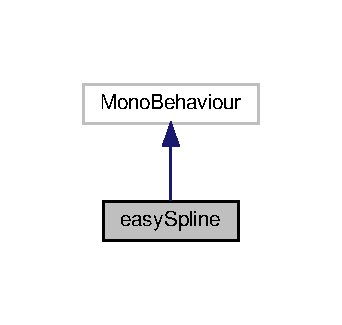
\includegraphics[width=164pt]{classeasySpline__inherit__graph}
\end{center}
\end{figure}


Collaboration diagram for easy\+Spline\+:\nopagebreak
\begin{figure}[H]
\begin{center}
\leavevmode
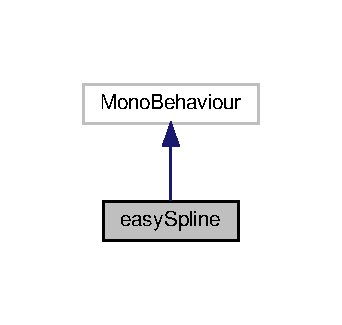
\includegraphics[width=164pt]{classeasySpline__coll__graph}
\end{center}
\end{figure}
\subsection*{Public Attributes}
\begin{DoxyCompactItemize}
\item 
float \hyperlink{classeasySpline_abb53dcde316e6ee14c45c1de1f033d4e}{x} = 1
\begin{DoxyCompactList}\small\item\em Length in x\end{DoxyCompactList}\item 
float \hyperlink{classeasySpline_a45bbb109c803b738a7c3a60711d9dc88}{z} = 1
\begin{DoxyCompactList}\small\item\em Length in z\end{DoxyCompactList}\item 
const float \hyperlink{classeasySpline_a15f0867bca07e689105eac1b61d92155}{borders\+FactorX} = 0.\+9f
\begin{DoxyCompactList}\small\item\em Ratio of x-\/coordinate borders. Only the borders\+Factor\+X-\/th will be used.\end{DoxyCompactList}\item 
const float \hyperlink{classeasySpline_a61234928f5a518ae8bb329f981efd903}{borders\+FactorZ} = 0.\+9f
\begin{DoxyCompactList}\small\item\em Ratio of y-\/coordinate borders. Only the borders\+Factor\+Z-\/th will be used.\end{DoxyCompactList}\end{DoxyCompactItemize}
\subsection*{Private Member Functions}
\begin{DoxyCompactItemize}
\item 
void \hyperlink{classeasySpline_aab9181ebea3a8c3ff1ee0503a282006f}{Start} ()
\begin{DoxyCompactList}\small\item\em Resize the Spline at the start of the simulation. \end{DoxyCompactList}\end{DoxyCompactItemize}
\subsection*{Private Attributes}
\begin{DoxyCompactItemize}
\item 
const float \hyperlink{classeasySpline_aa1cda6cd9ba7feb7251b526a320f0680}{length\+SplineX} = 5.\+770f
\begin{DoxyCompactList}\small\item\em X ratio used to resize the Spline at the requested size. Do not modify\end{DoxyCompactList}\item 
const float \hyperlink{classeasySpline_ada978fd8ee35f377dd8a46d6b736bf90}{length\+SplineZ} = 2.\+44f
\begin{DoxyCompactList}\small\item\em Z ratio used to resize the Spline at the requested size. Do not modify\end{DoxyCompactList}\end{DoxyCompactItemize}


\subsection{Detailed Description}
Interface to adapt the size of the Spline. 



\subsection{Member Function Documentation}
\mbox{\Hypertarget{classeasySpline_aab9181ebea3a8c3ff1ee0503a282006f}\label{classeasySpline_aab9181ebea3a8c3ff1ee0503a282006f}} 
\index{easy\+Spline@{easy\+Spline}!Start@{Start}}
\index{Start@{Start}!easy\+Spline@{easy\+Spline}}
\subsubsection{\texorpdfstring{Start()}{Start()}}
{\footnotesize\ttfamily void easy\+Spline.\+Start (\begin{DoxyParamCaption}{ }\end{DoxyParamCaption})\hspace{0.3cm}{\ttfamily [inline]}, {\ttfamily [private]}}



Resize the Spline at the start of the simulation. 



\subsection{Member Data Documentation}
\mbox{\Hypertarget{classeasySpline_a15f0867bca07e689105eac1b61d92155}\label{classeasySpline_a15f0867bca07e689105eac1b61d92155}} 
\index{easy\+Spline@{easy\+Spline}!borders\+FactorX@{borders\+FactorX}}
\index{borders\+FactorX@{borders\+FactorX}!easy\+Spline@{easy\+Spline}}
\subsubsection{\texorpdfstring{borders\+FactorX}{bordersFactorX}}
{\footnotesize\ttfamily const float easy\+Spline.\+borders\+FactorX = 0.\+9f}



Ratio of x-\/coordinate borders. Only the borders\+Factor\+X-\/th will be used.

\mbox{\Hypertarget{classeasySpline_a61234928f5a518ae8bb329f981efd903}\label{classeasySpline_a61234928f5a518ae8bb329f981efd903}} 
\index{easy\+Spline@{easy\+Spline}!borders\+FactorZ@{borders\+FactorZ}}
\index{borders\+FactorZ@{borders\+FactorZ}!easy\+Spline@{easy\+Spline}}
\subsubsection{\texorpdfstring{borders\+FactorZ}{bordersFactorZ}}
{\footnotesize\ttfamily const float easy\+Spline.\+borders\+FactorZ = 0.\+9f}



Ratio of y-\/coordinate borders. Only the borders\+Factor\+Z-\/th will be used.

\mbox{\Hypertarget{classeasySpline_aa1cda6cd9ba7feb7251b526a320f0680}\label{classeasySpline_aa1cda6cd9ba7feb7251b526a320f0680}} 
\index{easy\+Spline@{easy\+Spline}!length\+SplineX@{length\+SplineX}}
\index{length\+SplineX@{length\+SplineX}!easy\+Spline@{easy\+Spline}}
\subsubsection{\texorpdfstring{length\+SplineX}{lengthSplineX}}
{\footnotesize\ttfamily const float easy\+Spline.\+length\+SplineX = 5.\+770f\hspace{0.3cm}{\ttfamily [private]}}



X ratio used to resize the Spline at the requested size. Do not modify

\mbox{\Hypertarget{classeasySpline_ada978fd8ee35f377dd8a46d6b736bf90}\label{classeasySpline_ada978fd8ee35f377dd8a46d6b736bf90}} 
\index{easy\+Spline@{easy\+Spline}!length\+SplineZ@{length\+SplineZ}}
\index{length\+SplineZ@{length\+SplineZ}!easy\+Spline@{easy\+Spline}}
\subsubsection{\texorpdfstring{length\+SplineZ}{lengthSplineZ}}
{\footnotesize\ttfamily const float easy\+Spline.\+length\+SplineZ = 2.\+44f\hspace{0.3cm}{\ttfamily [private]}}



Z ratio used to resize the Spline at the requested size. Do not modify

\mbox{\Hypertarget{classeasySpline_abb53dcde316e6ee14c45c1de1f033d4e}\label{classeasySpline_abb53dcde316e6ee14c45c1de1f033d4e}} 
\index{easy\+Spline@{easy\+Spline}!x@{x}}
\index{x@{x}!easy\+Spline@{easy\+Spline}}
\subsubsection{\texorpdfstring{x}{x}}
{\footnotesize\ttfamily float easy\+Spline.\+x = 1}



Length in x

\mbox{\Hypertarget{classeasySpline_a45bbb109c803b738a7c3a60711d9dc88}\label{classeasySpline_a45bbb109c803b738a7c3a60711d9dc88}} 
\index{easy\+Spline@{easy\+Spline}!z@{z}}
\index{z@{z}!easy\+Spline@{easy\+Spline}}
\subsubsection{\texorpdfstring{z}{z}}
{\footnotesize\ttfamily float easy\+Spline.\+z = 1}



Length in z



The documentation for this class was generated from the following file\+:\begin{DoxyCompactItemize}
\item 
/root/\+Documents/\+Unity\+\_\+\+S\+T40/\+Suratram\+\_\+mixed\+Reality\+Simulator/\+Assets/\+Scripts/\+Bezier/\hyperlink{easySpline_8cs}{easy\+Spline.\+cs}\end{DoxyCompactItemize}

\hypertarget{classinformations}{}\section{informations Class Reference}
\label{classinformations}\index{informations@{informations}}


Class that displays some general informations on a Text component.  




Inheritance diagram for informations\+:\nopagebreak
\begin{figure}[H]
\begin{center}
\leavevmode
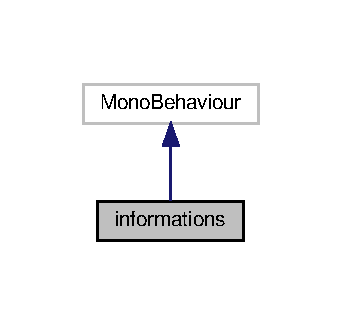
\includegraphics[width=164pt]{classinformations__inherit__graph}
\end{center}
\end{figure}


Collaboration diagram for informations\+:\nopagebreak
\begin{figure}[H]
\begin{center}
\leavevmode
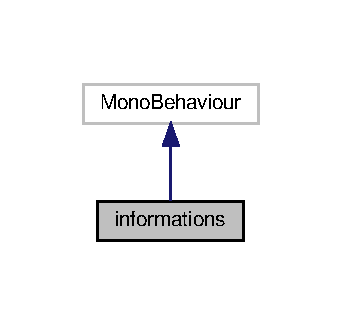
\includegraphics[width=164pt]{classinformations__coll__graph}
\end{center}
\end{figure}
\subsection*{Public Attributes}
\begin{DoxyCompactItemize}
\item 
float \hyperlink{classinformations_a61499fca827688fff9025d277f5cd589}{sampling\+Period} = 1
\begin{DoxyCompactList}\small\item\em The time needed for a refresh\end{DoxyCompactList}\end{DoxyCompactItemize}
\subsection*{Private Member Functions}
\begin{DoxyCompactItemize}
\item 
void \hyperlink{classinformations_adbca1b4eb5f7fc762725261b2469ee62}{Start} ()
\begin{DoxyCompactList}\small\item\em Initialization function. \end{DoxyCompactList}\item 
void \hyperlink{classinformations_a352b4a3e1670fd6c324ffe5659b76c5c}{Fixed\+Update} ()
\begin{DoxyCompactList}\small\item\em Updates the Text. \end{DoxyCompactList}\item 
void \hyperlink{classinformations_a6cbc72bf9a7cccdc906bc6ec0b0b870c}{update\+Text} (float vb, float ab, float vc, float ac, float interD)
\begin{DoxyCompactList}\small\item\em Displays on the Text the text with parameters. \end{DoxyCompactList}\end{DoxyCompactItemize}
\subsection*{Private Attributes}
\begin{DoxyCompactItemize}
\item 
float \hyperlink{classinformations_aab8401586ee1d9d587cdf9cf07611dbd}{time\+Start\+Sampling}
\begin{DoxyCompactList}\small\item\em An intern variable to store the time elapsed since the last refresh.\end{DoxyCompactList}\end{DoxyCompactItemize}


\subsection{Detailed Description}
Class that displays some general informations on a Text component. 



\subsection{Member Function Documentation}
\mbox{\Hypertarget{classinformations_a352b4a3e1670fd6c324ffe5659b76c5c}\label{classinformations_a352b4a3e1670fd6c324ffe5659b76c5c}} 
\index{informations@{informations}!Fixed\+Update@{Fixed\+Update}}
\index{Fixed\+Update@{Fixed\+Update}!informations@{informations}}
\subsubsection{\texorpdfstring{Fixed\+Update()}{FixedUpdate()}}
{\footnotesize\ttfamily void informations.\+Fixed\+Update (\begin{DoxyParamCaption}{ }\end{DoxyParamCaption})\hspace{0.3cm}{\ttfamily [inline]}, {\ttfamily [private]}}



Updates the Text. 

\mbox{\Hypertarget{classinformations_adbca1b4eb5f7fc762725261b2469ee62}\label{classinformations_adbca1b4eb5f7fc762725261b2469ee62}} 
\index{informations@{informations}!Start@{Start}}
\index{Start@{Start}!informations@{informations}}
\subsubsection{\texorpdfstring{Start()}{Start()}}
{\footnotesize\ttfamily void informations.\+Start (\begin{DoxyParamCaption}{ }\end{DoxyParamCaption})\hspace{0.3cm}{\ttfamily [inline]}, {\ttfamily [private]}}



Initialization function. 

\mbox{\Hypertarget{classinformations_a6cbc72bf9a7cccdc906bc6ec0b0b870c}\label{classinformations_a6cbc72bf9a7cccdc906bc6ec0b0b870c}} 
\index{informations@{informations}!update\+Text@{update\+Text}}
\index{update\+Text@{update\+Text}!informations@{informations}}
\subsubsection{\texorpdfstring{update\+Text()}{updateText()}}
{\footnotesize\ttfamily void informations.\+update\+Text (\begin{DoxyParamCaption}\item[{float}]{vb,  }\item[{float}]{ab,  }\item[{float}]{vc,  }\item[{float}]{ac,  }\item[{float}]{interD }\end{DoxyParamCaption})\hspace{0.3cm}{\ttfamily [inline]}, {\ttfamily [private]}}



Displays on the Text the text with parameters. 


\begin{DoxyParams}{Parameters}
{\em vb} & The velocity of the bus.\\
\hline
{\em ab} & The acceleration of the bus.\\
\hline
{\em vc} & The velocity of the car.\\
\hline
{\em ac} & The acceleration of the car.\\
\hline
{\em interD} & The inter-\/distance between the two vehicles.\\
\hline
\end{DoxyParams}


\subsection{Member Data Documentation}
\mbox{\Hypertarget{classinformations_a61499fca827688fff9025d277f5cd589}\label{classinformations_a61499fca827688fff9025d277f5cd589}} 
\index{informations@{informations}!sampling\+Period@{sampling\+Period}}
\index{sampling\+Period@{sampling\+Period}!informations@{informations}}
\subsubsection{\texorpdfstring{sampling\+Period}{samplingPeriod}}
{\footnotesize\ttfamily float informations.\+sampling\+Period = 1}



The time needed for a refresh

\mbox{\Hypertarget{classinformations_aab8401586ee1d9d587cdf9cf07611dbd}\label{classinformations_aab8401586ee1d9d587cdf9cf07611dbd}} 
\index{informations@{informations}!time\+Start\+Sampling@{time\+Start\+Sampling}}
\index{time\+Start\+Sampling@{time\+Start\+Sampling}!informations@{informations}}
\subsubsection{\texorpdfstring{time\+Start\+Sampling}{timeStartSampling}}
{\footnotesize\ttfamily float informations.\+time\+Start\+Sampling\hspace{0.3cm}{\ttfamily [private]}}



An intern variable to store the time elapsed since the last refresh.



The documentation for this class was generated from the following file\+:\begin{DoxyCompactItemize}
\item 
/root/\+Documents/\+Unity\+\_\+\+S\+T40/\+Suratram\+\_\+mixed\+Reality\+Simulator/\+Assets/\+Scripts/\+U\+I/\hyperlink{informations_8cs}{informations.\+cs}\end{DoxyCompactItemize}

\hypertarget{classLine}{}\section{Line Class Reference}
\label{classLine}\index{Line@{Line}}


Inheritance diagram for Line\+:\nopagebreak
\begin{figure}[H]
\begin{center}
\leavevmode
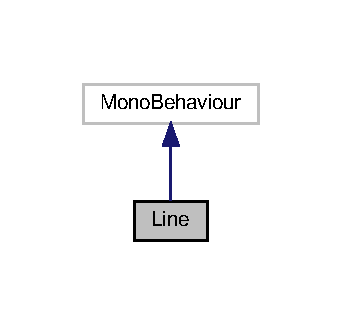
\includegraphics[width=164pt]{classLine__inherit__graph}
\end{center}
\end{figure}


Collaboration diagram for Line\+:\nopagebreak
\begin{figure}[H]
\begin{center}
\leavevmode
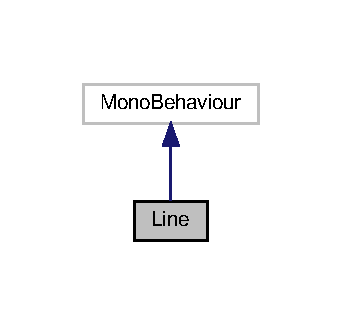
\includegraphics[width=164pt]{classLine__coll__graph}
\end{center}
\end{figure}
\subsection*{Public Attributes}
\begin{DoxyCompactItemize}
\item 
Vector3 \hyperlink{classLine_a20d5ecabee2113e42017734b748b485d}{p0}
\end{DoxyCompactItemize}
\subsection*{Private Attributes}
\begin{DoxyCompactItemize}
\item 
Vector3 \hyperlink{classLine_aaecb847629b70b917115e59873531cdb}{p1}
\end{DoxyCompactItemize}


\subsection{Member Data Documentation}
\mbox{\Hypertarget{classLine_a20d5ecabee2113e42017734b748b485d}\label{classLine_a20d5ecabee2113e42017734b748b485d}} 
\index{Line@{Line}!p0@{p0}}
\index{p0@{p0}!Line@{Line}}
\subsubsection{\texorpdfstring{p0}{p0}}
{\footnotesize\ttfamily Vector3 Line.\+p0}

\mbox{\Hypertarget{classLine_aaecb847629b70b917115e59873531cdb}\label{classLine_aaecb847629b70b917115e59873531cdb}} 
\index{Line@{Line}!p1@{p1}}
\index{p1@{p1}!Line@{Line}}
\subsubsection{\texorpdfstring{p1}{p1}}
{\footnotesize\ttfamily Vector3 Line.\+p1\hspace{0.3cm}{\ttfamily [private]}}



The documentation for this class was generated from the following file\+:\begin{DoxyCompactItemize}
\item 
/root/\+Documents/\+Unity\+\_\+\+S\+T40/\+Suratram\+\_\+mixed\+Reality\+Simulator/\+Assets/\+Scripts/\+Bezier/\hyperlink{Line_8cs}{Line.\+cs}\end{DoxyCompactItemize}

\hypertarget{classLineInspector}{}\section{Line\+Inspector Class Reference}
\label{classLineInspector}\index{Line\+Inspector@{Line\+Inspector}}


Inheritance diagram for Line\+Inspector\+:\nopagebreak
\begin{figure}[H]
\begin{center}
\leavevmode
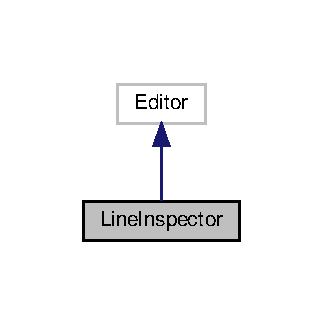
\includegraphics[width=155pt]{classLineInspector__inherit__graph}
\end{center}
\end{figure}


Collaboration diagram for Line\+Inspector\+:\nopagebreak
\begin{figure}[H]
\begin{center}
\leavevmode
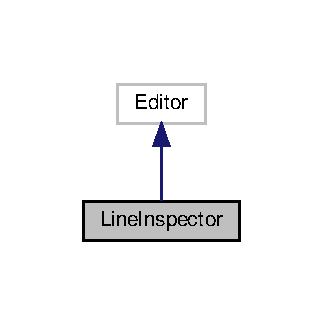
\includegraphics[width=155pt]{classLineInspector__coll__graph}
\end{center}
\end{figure}
\subsection*{Private Member Functions}
\begin{DoxyCompactItemize}
\item 
void \hyperlink{classLineInspector_a5d0b1541e2e3172637349afe61a1d1a3}{On\+Scene\+G\+UI} ()
\end{DoxyCompactItemize}


\subsection{Member Function Documentation}
\mbox{\Hypertarget{classLineInspector_a5d0b1541e2e3172637349afe61a1d1a3}\label{classLineInspector_a5d0b1541e2e3172637349afe61a1d1a3}} 
\index{Line\+Inspector@{Line\+Inspector}!On\+Scene\+G\+UI@{On\+Scene\+G\+UI}}
\index{On\+Scene\+G\+UI@{On\+Scene\+G\+UI}!Line\+Inspector@{Line\+Inspector}}
\subsubsection{\texorpdfstring{On\+Scene\+G\+U\+I()}{OnSceneGUI()}}
{\footnotesize\ttfamily void Line\+Inspector.\+On\+Scene\+G\+UI (\begin{DoxyParamCaption}{ }\end{DoxyParamCaption})\hspace{0.3cm}{\ttfamily [inline]}, {\ttfamily [private]}}



The documentation for this class was generated from the following file\+:\begin{DoxyCompactItemize}
\item 
/root/\+Documents/\+Unity\+\_\+\+S\+T40/\+Suratram\+\_\+mixed\+Reality\+Simulator/\+Assets/\+Scripts/\+Bezier/\+Editor/\hyperlink{LineInspector_8cs}{Line\+Inspector.\+cs}\end{DoxyCompactItemize}

\hypertarget{classmonitoring}{}\section{monitoring Class Reference}
\label{classmonitoring}\index{monitoring@{monitoring}}


This class monitors, by retrieving differents informations in the scene.  




Inheritance diagram for monitoring\+:\nopagebreak
\begin{figure}[H]
\begin{center}
\leavevmode
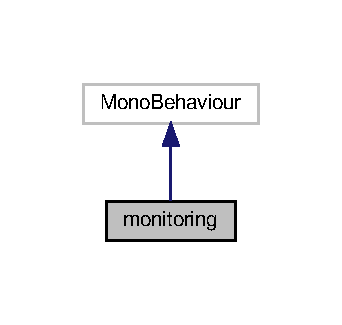
\includegraphics[width=164pt]{classmonitoring__inherit__graph}
\end{center}
\end{figure}


Collaboration diagram for monitoring\+:\nopagebreak
\begin{figure}[H]
\begin{center}
\leavevmode
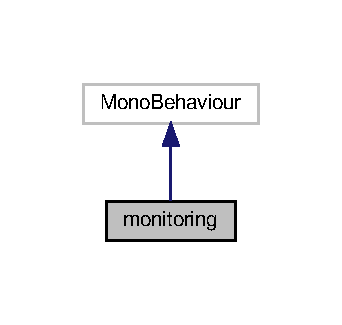
\includegraphics[width=164pt]{classmonitoring__coll__graph}
\end{center}
\end{figure}
\subsection*{Public Attributes}
\begin{DoxyCompactItemize}
\item 
float \hyperlink{classmonitoring_a20213a8bca2c7713ea994a8f0625e810}{sampling\+Period} = 1f
\begin{DoxyCompactList}\small\item\em The time for every value update\end{DoxyCompactList}\item 
\hyperlink{classmonitoring_a4a225f8529921b2f6b38156cf3b296cf}{Vector3}
\begin{DoxyCompactList}\small\item\em Array of a 2-\/tuple containing both position and time stamp of this data. Circular override of values.\end{DoxyCompactList}\end{DoxyCompactItemize}
\subsection*{Properties}
\begin{DoxyCompactItemize}
\item 
static float \hyperlink{classmonitoring_aa1b0006663cd5ba0712be4d8a7456638}{velocity\+Bus}\hspace{0.3cm}{\ttfamily  \mbox{[}get, private set\mbox{]}}
\begin{DoxyCompactList}\small\item\em The velocity of the bus obtained after the data has been filtered.\end{DoxyCompactList}\item 
static float \hyperlink{classmonitoring_aa6614515aa744b660b183fef95c22dbd}{velocity\+Car}\hspace{0.3cm}{\ttfamily  \mbox{[}get, private set\mbox{]}}
\begin{DoxyCompactList}\small\item\em The velocity of the car obtained after the data has been filtered.\end{DoxyCompactList}\item 
static float \hyperlink{classmonitoring_aa570e9f19b8dac133c43bb5f3c1ae2a3}{acceleration\+Bus}\hspace{0.3cm}{\ttfamily  \mbox{[}get, private set\mbox{]}}
\begin{DoxyCompactList}\small\item\em The acceleration of the bus obtained after the data has been filtered.\end{DoxyCompactList}\item 
static float \hyperlink{classmonitoring_aaaf8354f9953bda4e43e4f0b66923467}{acceleration\+Car}\hspace{0.3cm}{\ttfamily  \mbox{[}get, private set\mbox{]}}
\begin{DoxyCompactList}\small\item\em The acceleration of the car obtained after the data has been filtered.\end{DoxyCompactList}\item 
float \mbox{[}$\,$\mbox{]} \hyperlink{classmonitoring_a9fdc2f6e44aff0f03ff05a1cfa2f9d79}{pos\+Bus\+Arr}\hspace{0.3cm}{\ttfamily  \mbox{[}get, private set\mbox{]}}
\item 
static float \hyperlink{classmonitoring_a8e2c4ef74df749bdc13e8a29c066eb6b}{inter\+Distance}\hspace{0.3cm}{\ttfamily  \mbox{[}get, private set\mbox{]}}
\begin{DoxyCompactList}\small\item\em The inter-\/distance obtained after the data has been filtered.\end{DoxyCompactList}\end{DoxyCompactItemize}
\subsection*{Private Member Functions}
\begin{DoxyCompactItemize}
\item 
void \hyperlink{classmonitoring_a4aa220d0178d2b204e8039855c412c30}{Start} ()
\begin{DoxyCompactList}\small\item\em Initialisation of the class. \end{DoxyCompactList}\item 
void \hyperlink{classmonitoring_a257af7f7bd0d01b91dc5d34f85743b5f}{Fixed\+Update} ()
\begin{DoxyCompactList}\small\item\em Function that updates every frame the data. And every \textquotesingle{}sampling\+Period\textquotesingle{} it publishs the filtered data in public variables. \end{DoxyCompactList}\item 
float \hyperlink{classmonitoring_a02b9ad38b7160a01547d1540d3ced5a2}{average} (float\mbox{[}$\,$\mbox{]} arr, int \hyperlink{classmonitoring_a6f24f8f72c806c9afab0e3de87636a27}{index\+Sampling})
\begin{DoxyCompactList}\small\item\em Function that computes the average of the {\ttfamily index\+Sampling}-\/th elements of a float array. \end{DoxyCompactList}\item 
\hyperlink{classmonitoring_a4a225f8529921b2f6b38156cf3b296cf}{Vector3} \hyperlink{classmonitoring_a8b3badd3272bcdef5a3f438db1dbde7f}{average} (\hyperlink{classmonitoring_a4a225f8529921b2f6b38156cf3b296cf}{Vector3}\mbox{[}$\,$\mbox{]} arr, int \hyperlink{classmonitoring_a6f24f8f72c806c9afab0e3de87636a27}{index\+Sampling})
\begin{DoxyCompactList}\small\item\em Function that computes the average of the {\ttfamily index\+Sampling}-\/th elements of a {\ttfamily Vector3} array. \end{DoxyCompactList}\item 
void \hyperlink{classmonitoring_af09a1f1c17d9523758c57e7808afc81d}{array\+Shift\+Right$<$ T $>$} (T\mbox{[}$\,$\mbox{]} arr)
\begin{DoxyCompactList}\small\item\em Function that shifts every element of a array to the right. \end{DoxyCompactList}\end{DoxyCompactItemize}
\subsection*{Private Attributes}
\begin{DoxyCompactItemize}
\item 
const int \hyperlink{classmonitoring_ac4fadca0a90c03c7cd175155ead8df0f}{nb\+Data\+Max} = 10000
\begin{DoxyCompactList}\small\item\em The max number of data informations that can be stored.\end{DoxyCompactList}\item 
float \hyperlink{classmonitoring_a15b5bc6036048bde3e57edcbf53f6bc3}{time\+Start\+Sampling}
\begin{DoxyCompactList}\small\item\em Variable to store the elapsed time since the last data merge.\end{DoxyCompactList}\item 
int \hyperlink{classmonitoring_a6f24f8f72c806c9afab0e3de87636a27}{index\+Sampling}
\begin{DoxyCompactList}\small\item\em The current number of data sample that has been gathered but not merged.\end{DoxyCompactList}\item 
\hyperlink{classmonitoring_a4a225f8529921b2f6b38156cf3b296cf}{Vector3} \mbox{[}$\,$\mbox{]} \hyperlink{classmonitoring_a37b82c6f5aad1407bf7d68fa141d5c2e}{tmp\+Pos\+Bus\+Arr}
\begin{DoxyCompactList}\small\item\em The raw data of bus positon. Filled over time.\end{DoxyCompactList}\item 
\hyperlink{classmonitoring_a4a225f8529921b2f6b38156cf3b296cf}{Vector3} \mbox{[}$\,$\mbox{]} \hyperlink{classmonitoring_ac92542c319fc95a3b1126dba86a675de}{tmp\+Pos\+Car\+Arr}
\begin{DoxyCompactList}\small\item\em The raw data of car positon. Filled over time.\end{DoxyCompactList}\item 
float \mbox{[}$\,$\mbox{]} \hyperlink{classmonitoring_ade021e7adddbe127c8dd4413fac36483}{velocity\+Bus\+Arr}
\begin{DoxyCompactList}\small\item\em The raw data of bus velocity. Filled over time.\end{DoxyCompactList}\item 
float \mbox{[}$\,$\mbox{]} \hyperlink{classmonitoring_ad1c1a9788538be54e5cc7cf23d11424e}{velocity\+Car\+Arr}
\begin{DoxyCompactList}\small\item\em The raw data of car velocity. Filled over time.\end{DoxyCompactList}\item 
float \mbox{[}$\,$\mbox{]} \hyperlink{classmonitoring_acf6692391e841215c8dbeec584100901}{acceleration\+Bus\+Arr}
\begin{DoxyCompactList}\small\item\em The raw data of bus acceleration. Filled over time.\end{DoxyCompactList}\item 
float \mbox{[}$\,$\mbox{]} \hyperlink{classmonitoring_a1dba43f12e646b6d346eaa1a406f6c68}{acceleration\+Car\+Arr}
\begin{DoxyCompactList}\small\item\em The raw data of car acceleration. Filled over time.\end{DoxyCompactList}\item 
float \mbox{[}$\,$\mbox{]} \hyperlink{classmonitoring_a02f147c189ffeb8d4bd454ad353d98df}{inter\+Distance\+Arr}
\begin{DoxyCompactList}\small\item\em The raw data of the inter-\/distance. Filled over time.\end{DoxyCompactList}\item 
double \mbox{[}$\,$\mbox{]} \hyperlink{classmonitoring_aa93593cba4aa6835e47e3714106e0afb}{array\+Delta\+Time}
\begin{DoxyCompactList}\small\item\em The raw data of the time elapsed between every sample. Filled over time.\end{DoxyCompactList}\end{DoxyCompactItemize}


\subsection{Detailed Description}
This class monitors, by retrieving differents informations in the scene. 



\subsection{Member Function Documentation}
\mbox{\Hypertarget{classmonitoring_af09a1f1c17d9523758c57e7808afc81d}\label{classmonitoring_af09a1f1c17d9523758c57e7808afc81d}} 
\index{monitoring@{monitoring}!array\+Shift\+Right$<$ T $>$@{array\+Shift\+Right$<$ T $>$}}
\index{array\+Shift\+Right$<$ T $>$@{array\+Shift\+Right$<$ T $>$}!monitoring@{monitoring}}
\subsubsection{\texorpdfstring{array\+Shift\+Right$<$ T $>$()}{arrayShiftRight< T >()}}
{\footnotesize\ttfamily void monitoring.\+array\+Shift\+Right$<$ T $>$ (\begin{DoxyParamCaption}\item[{T \mbox{[}$\,$\mbox{]}}]{arr }\end{DoxyParamCaption})\hspace{0.3cm}{\ttfamily [inline]}, {\ttfamily [private]}}



Function that shifts every element of a array to the right. 


\begin{DoxyParams}{Parameters}
{\em arr} & Source array of elements, type of template {\ttfamily T}\\
\hline
\end{DoxyParams}


Initialize the {\ttfamily 0-\/th} element with the default {\ttfamily T} value.\mbox{\Hypertarget{classmonitoring_a02b9ad38b7160a01547d1540d3ced5a2}\label{classmonitoring_a02b9ad38b7160a01547d1540d3ced5a2}} 
\index{monitoring@{monitoring}!average@{average}}
\index{average@{average}!monitoring@{monitoring}}
\subsubsection{\texorpdfstring{average()}{average()}\hspace{0.1cm}{\footnotesize\ttfamily [1/2]}}
{\footnotesize\ttfamily float monitoring.\+average (\begin{DoxyParamCaption}\item[{float \mbox{[}$\,$\mbox{]}}]{arr,  }\item[{int}]{index\+Sampling }\end{DoxyParamCaption})\hspace{0.3cm}{\ttfamily [inline]}, {\ttfamily [private]}}



Function that computes the average of the {\ttfamily index\+Sampling}-\/th elements of a float array. 


\begin{DoxyParams}{Parameters}
{\em arr} & The float array source\\
\hline
\end{DoxyParams}
\begin{DoxyReturn}{Returns}
The average value
\end{DoxyReturn}
\mbox{\Hypertarget{classmonitoring_a8b3badd3272bcdef5a3f438db1dbde7f}\label{classmonitoring_a8b3badd3272bcdef5a3f438db1dbde7f}} 
\index{monitoring@{monitoring}!average@{average}}
\index{average@{average}!monitoring@{monitoring}}
\subsubsection{\texorpdfstring{average()}{average()}\hspace{0.1cm}{\footnotesize\ttfamily [2/2]}}
{\footnotesize\ttfamily \hyperlink{classmonitoring_a4a225f8529921b2f6b38156cf3b296cf}{Vector3} monitoring.\+average (\begin{DoxyParamCaption}\item[{\hyperlink{classmonitoring_a4a225f8529921b2f6b38156cf3b296cf}{Vector3} \mbox{[}$\,$\mbox{]}}]{arr,  }\item[{int}]{index\+Sampling }\end{DoxyParamCaption})\hspace{0.3cm}{\ttfamily [inline]}, {\ttfamily [private]}}



Function that computes the average of the {\ttfamily index\+Sampling}-\/th elements of a {\ttfamily Vector3} array. 


\begin{DoxyParams}{Parameters}
{\em arr} & The Vector3 array source\\
\hline
\end{DoxyParams}
\begin{DoxyReturn}{Returns}
The average value, stored in a {\ttfamily Vector3}
\end{DoxyReturn}
\mbox{\Hypertarget{classmonitoring_a257af7f7bd0d01b91dc5d34f85743b5f}\label{classmonitoring_a257af7f7bd0d01b91dc5d34f85743b5f}} 
\index{monitoring@{monitoring}!Fixed\+Update@{Fixed\+Update}}
\index{Fixed\+Update@{Fixed\+Update}!monitoring@{monitoring}}
\subsubsection{\texorpdfstring{Fixed\+Update()}{FixedUpdate()}}
{\footnotesize\ttfamily void monitoring.\+Fixed\+Update (\begin{DoxyParamCaption}{ }\end{DoxyParamCaption})\hspace{0.3cm}{\ttfamily [inline]}, {\ttfamily [private]}}



Function that updates every frame the data. And every \textquotesingle{}sampling\+Period\textquotesingle{} it publishs the filtered data in public variables. 

\mbox{\Hypertarget{classmonitoring_a4aa220d0178d2b204e8039855c412c30}\label{classmonitoring_a4aa220d0178d2b204e8039855c412c30}} 
\index{monitoring@{monitoring}!Start@{Start}}
\index{Start@{Start}!monitoring@{monitoring}}
\subsubsection{\texorpdfstring{Start()}{Start()}}
{\footnotesize\ttfamily void monitoring.\+Start (\begin{DoxyParamCaption}{ }\end{DoxyParamCaption})\hspace{0.3cm}{\ttfamily [inline]}, {\ttfamily [private]}}



Initialisation of the class. 



\subsection{Member Data Documentation}
\mbox{\Hypertarget{classmonitoring_acf6692391e841215c8dbeec584100901}\label{classmonitoring_acf6692391e841215c8dbeec584100901}} 
\index{monitoring@{monitoring}!acceleration\+Bus\+Arr@{acceleration\+Bus\+Arr}}
\index{acceleration\+Bus\+Arr@{acceleration\+Bus\+Arr}!monitoring@{monitoring}}
\subsubsection{\texorpdfstring{acceleration\+Bus\+Arr}{accelerationBusArr}}
{\footnotesize\ttfamily float \mbox{[}$\,$\mbox{]} monitoring.\+acceleration\+Bus\+Arr\hspace{0.3cm}{\ttfamily [private]}}



The raw data of bus acceleration. Filled over time.

\mbox{\Hypertarget{classmonitoring_a1dba43f12e646b6d346eaa1a406f6c68}\label{classmonitoring_a1dba43f12e646b6d346eaa1a406f6c68}} 
\index{monitoring@{monitoring}!acceleration\+Car\+Arr@{acceleration\+Car\+Arr}}
\index{acceleration\+Car\+Arr@{acceleration\+Car\+Arr}!monitoring@{monitoring}}
\subsubsection{\texorpdfstring{acceleration\+Car\+Arr}{accelerationCarArr}}
{\footnotesize\ttfamily float \mbox{[}$\,$\mbox{]} monitoring.\+acceleration\+Car\+Arr\hspace{0.3cm}{\ttfamily [private]}}



The raw data of car acceleration. Filled over time.

\mbox{\Hypertarget{classmonitoring_aa93593cba4aa6835e47e3714106e0afb}\label{classmonitoring_aa93593cba4aa6835e47e3714106e0afb}} 
\index{monitoring@{monitoring}!array\+Delta\+Time@{array\+Delta\+Time}}
\index{array\+Delta\+Time@{array\+Delta\+Time}!monitoring@{monitoring}}
\subsubsection{\texorpdfstring{array\+Delta\+Time}{arrayDeltaTime}}
{\footnotesize\ttfamily double \mbox{[}$\,$\mbox{]} monitoring.\+array\+Delta\+Time\hspace{0.3cm}{\ttfamily [private]}}



The raw data of the time elapsed between every sample. Filled over time.

\mbox{\Hypertarget{classmonitoring_a6f24f8f72c806c9afab0e3de87636a27}\label{classmonitoring_a6f24f8f72c806c9afab0e3de87636a27}} 
\index{monitoring@{monitoring}!index\+Sampling@{index\+Sampling}}
\index{index\+Sampling@{index\+Sampling}!monitoring@{monitoring}}
\subsubsection{\texorpdfstring{index\+Sampling}{indexSampling}}
{\footnotesize\ttfamily int monitoring.\+index\+Sampling\hspace{0.3cm}{\ttfamily [private]}}



The current number of data sample that has been gathered but not merged.

\mbox{\Hypertarget{classmonitoring_a02f147c189ffeb8d4bd454ad353d98df}\label{classmonitoring_a02f147c189ffeb8d4bd454ad353d98df}} 
\index{monitoring@{monitoring}!inter\+Distance\+Arr@{inter\+Distance\+Arr}}
\index{inter\+Distance\+Arr@{inter\+Distance\+Arr}!monitoring@{monitoring}}
\subsubsection{\texorpdfstring{inter\+Distance\+Arr}{interDistanceArr}}
{\footnotesize\ttfamily float \mbox{[}$\,$\mbox{]} monitoring.\+inter\+Distance\+Arr\hspace{0.3cm}{\ttfamily [private]}}



The raw data of the inter-\/distance. Filled over time.

\mbox{\Hypertarget{classmonitoring_ac4fadca0a90c03c7cd175155ead8df0f}\label{classmonitoring_ac4fadca0a90c03c7cd175155ead8df0f}} 
\index{monitoring@{monitoring}!nb\+Data\+Max@{nb\+Data\+Max}}
\index{nb\+Data\+Max@{nb\+Data\+Max}!monitoring@{monitoring}}
\subsubsection{\texorpdfstring{nb\+Data\+Max}{nbDataMax}}
{\footnotesize\ttfamily const int monitoring.\+nb\+Data\+Max = 10000\hspace{0.3cm}{\ttfamily [private]}}



The max number of data informations that can be stored.

\mbox{\Hypertarget{classmonitoring_a20213a8bca2c7713ea994a8f0625e810}\label{classmonitoring_a20213a8bca2c7713ea994a8f0625e810}} 
\index{monitoring@{monitoring}!sampling\+Period@{sampling\+Period}}
\index{sampling\+Period@{sampling\+Period}!monitoring@{monitoring}}
\subsubsection{\texorpdfstring{sampling\+Period}{samplingPeriod}}
{\footnotesize\ttfamily float monitoring.\+sampling\+Period = 1f}



The time for every value update

\mbox{\Hypertarget{classmonitoring_a15b5bc6036048bde3e57edcbf53f6bc3}\label{classmonitoring_a15b5bc6036048bde3e57edcbf53f6bc3}} 
\index{monitoring@{monitoring}!time\+Start\+Sampling@{time\+Start\+Sampling}}
\index{time\+Start\+Sampling@{time\+Start\+Sampling}!monitoring@{monitoring}}
\subsubsection{\texorpdfstring{time\+Start\+Sampling}{timeStartSampling}}
{\footnotesize\ttfamily float monitoring.\+time\+Start\+Sampling\hspace{0.3cm}{\ttfamily [private]}}



Variable to store the elapsed time since the last data merge.

\mbox{\Hypertarget{classmonitoring_a37b82c6f5aad1407bf7d68fa141d5c2e}\label{classmonitoring_a37b82c6f5aad1407bf7d68fa141d5c2e}} 
\index{monitoring@{monitoring}!tmp\+Pos\+Bus\+Arr@{tmp\+Pos\+Bus\+Arr}}
\index{tmp\+Pos\+Bus\+Arr@{tmp\+Pos\+Bus\+Arr}!monitoring@{monitoring}}
\subsubsection{\texorpdfstring{tmp\+Pos\+Bus\+Arr}{tmpPosBusArr}}
{\footnotesize\ttfamily \hyperlink{classmonitoring_a4a225f8529921b2f6b38156cf3b296cf}{Vector3} \mbox{[}$\,$\mbox{]} monitoring.\+tmp\+Pos\+Bus\+Arr\hspace{0.3cm}{\ttfamily [private]}}



The raw data of bus positon. Filled over time.

\mbox{\Hypertarget{classmonitoring_ac92542c319fc95a3b1126dba86a675de}\label{classmonitoring_ac92542c319fc95a3b1126dba86a675de}} 
\index{monitoring@{monitoring}!tmp\+Pos\+Car\+Arr@{tmp\+Pos\+Car\+Arr}}
\index{tmp\+Pos\+Car\+Arr@{tmp\+Pos\+Car\+Arr}!monitoring@{monitoring}}
\subsubsection{\texorpdfstring{tmp\+Pos\+Car\+Arr}{tmpPosCarArr}}
{\footnotesize\ttfamily \hyperlink{classmonitoring_a4a225f8529921b2f6b38156cf3b296cf}{Vector3} \mbox{[}$\,$\mbox{]} monitoring.\+tmp\+Pos\+Car\+Arr\hspace{0.3cm}{\ttfamily [private]}}



The raw data of car positon. Filled over time.

\mbox{\Hypertarget{classmonitoring_a4a225f8529921b2f6b38156cf3b296cf}\label{classmonitoring_a4a225f8529921b2f6b38156cf3b296cf}} 
\index{monitoring@{monitoring}!Vector3@{Vector3}}
\index{Vector3@{Vector3}!monitoring@{monitoring}}
\subsubsection{\texorpdfstring{Vector3}{Vector3}}
{\footnotesize\ttfamily monitoring.\+Vector3}



Array of a 2-\/tuple containing both position and time stamp of this data. Circular override of values.

\mbox{\Hypertarget{classmonitoring_ade021e7adddbe127c8dd4413fac36483}\label{classmonitoring_ade021e7adddbe127c8dd4413fac36483}} 
\index{monitoring@{monitoring}!velocity\+Bus\+Arr@{velocity\+Bus\+Arr}}
\index{velocity\+Bus\+Arr@{velocity\+Bus\+Arr}!monitoring@{monitoring}}
\subsubsection{\texorpdfstring{velocity\+Bus\+Arr}{velocityBusArr}}
{\footnotesize\ttfamily float \mbox{[}$\,$\mbox{]} monitoring.\+velocity\+Bus\+Arr\hspace{0.3cm}{\ttfamily [private]}}



The raw data of bus velocity. Filled over time.

\mbox{\Hypertarget{classmonitoring_ad1c1a9788538be54e5cc7cf23d11424e}\label{classmonitoring_ad1c1a9788538be54e5cc7cf23d11424e}} 
\index{monitoring@{monitoring}!velocity\+Car\+Arr@{velocity\+Car\+Arr}}
\index{velocity\+Car\+Arr@{velocity\+Car\+Arr}!monitoring@{monitoring}}
\subsubsection{\texorpdfstring{velocity\+Car\+Arr}{velocityCarArr}}
{\footnotesize\ttfamily float \mbox{[}$\,$\mbox{]} monitoring.\+velocity\+Car\+Arr\hspace{0.3cm}{\ttfamily [private]}}



The raw data of car velocity. Filled over time.



\subsection{Property Documentation}
\mbox{\Hypertarget{classmonitoring_aa570e9f19b8dac133c43bb5f3c1ae2a3}\label{classmonitoring_aa570e9f19b8dac133c43bb5f3c1ae2a3}} 
\index{monitoring@{monitoring}!acceleration\+Bus@{acceleration\+Bus}}
\index{acceleration\+Bus@{acceleration\+Bus}!monitoring@{monitoring}}
\subsubsection{\texorpdfstring{acceleration\+Bus}{accelerationBus}}
{\footnotesize\ttfamily float monitoring.\+acceleration\+Bus\hspace{0.3cm}{\ttfamily [static]}, {\ttfamily [get]}, {\ttfamily [private set]}}



The acceleration of the bus obtained after the data has been filtered.

\mbox{\Hypertarget{classmonitoring_aaaf8354f9953bda4e43e4f0b66923467}\label{classmonitoring_aaaf8354f9953bda4e43e4f0b66923467}} 
\index{monitoring@{monitoring}!acceleration\+Car@{acceleration\+Car}}
\index{acceleration\+Car@{acceleration\+Car}!monitoring@{monitoring}}
\subsubsection{\texorpdfstring{acceleration\+Car}{accelerationCar}}
{\footnotesize\ttfamily float monitoring.\+acceleration\+Car\hspace{0.3cm}{\ttfamily [static]}, {\ttfamily [get]}, {\ttfamily [private set]}}



The acceleration of the car obtained after the data has been filtered.

\mbox{\Hypertarget{classmonitoring_a8e2c4ef74df749bdc13e8a29c066eb6b}\label{classmonitoring_a8e2c4ef74df749bdc13e8a29c066eb6b}} 
\index{monitoring@{monitoring}!inter\+Distance@{inter\+Distance}}
\index{inter\+Distance@{inter\+Distance}!monitoring@{monitoring}}
\subsubsection{\texorpdfstring{inter\+Distance}{interDistance}}
{\footnotesize\ttfamily float monitoring.\+inter\+Distance\hspace{0.3cm}{\ttfamily [static]}, {\ttfamily [get]}, {\ttfamily [private set]}}



The inter-\/distance obtained after the data has been filtered.

\mbox{\Hypertarget{classmonitoring_a9fdc2f6e44aff0f03ff05a1cfa2f9d79}\label{classmonitoring_a9fdc2f6e44aff0f03ff05a1cfa2f9d79}} 
\index{monitoring@{monitoring}!pos\+Bus\+Arr@{pos\+Bus\+Arr}}
\index{pos\+Bus\+Arr@{pos\+Bus\+Arr}!monitoring@{monitoring}}
\subsubsection{\texorpdfstring{pos\+Bus\+Arr}{posBusArr}}
{\footnotesize\ttfamily float \mbox{[}$\,$\mbox{]} monitoring.\+pos\+Bus\+Arr\hspace{0.3cm}{\ttfamily [get]}, {\ttfamily [private set]}, {\ttfamily [private]}}

\mbox{\Hypertarget{classmonitoring_aa1b0006663cd5ba0712be4d8a7456638}\label{classmonitoring_aa1b0006663cd5ba0712be4d8a7456638}} 
\index{monitoring@{monitoring}!velocity\+Bus@{velocity\+Bus}}
\index{velocity\+Bus@{velocity\+Bus}!monitoring@{monitoring}}
\subsubsection{\texorpdfstring{velocity\+Bus}{velocityBus}}
{\footnotesize\ttfamily float monitoring.\+velocity\+Bus\hspace{0.3cm}{\ttfamily [static]}, {\ttfamily [get]}, {\ttfamily [private set]}}



The velocity of the bus obtained after the data has been filtered.

\mbox{\Hypertarget{classmonitoring_aa6614515aa744b660b183fef95c22dbd}\label{classmonitoring_aa6614515aa744b660b183fef95c22dbd}} 
\index{monitoring@{monitoring}!velocity\+Car@{velocity\+Car}}
\index{velocity\+Car@{velocity\+Car}!monitoring@{monitoring}}
\subsubsection{\texorpdfstring{velocity\+Car}{velocityCar}}
{\footnotesize\ttfamily float monitoring.\+velocity\+Car\hspace{0.3cm}{\ttfamily [static]}, {\ttfamily [get]}, {\ttfamily [private set]}}



The velocity of the car obtained after the data has been filtered.



The documentation for this class was generated from the following file\+:\begin{DoxyCompactItemize}
\item 
/root/\+Documents/\+Unity\+\_\+\+S\+T40/\+Suratram\+\_\+mixed\+Reality\+Simulator/\+Assets/\+Scripts/\hyperlink{monitoring_8cs}{monitoring.\+cs}\end{DoxyCompactItemize}

\hypertarget{classSplineWalker}{}\section{Spline\+Walker Class Reference}
\label{classSplineWalker}\index{Spline\+Walker@{Spline\+Walker}}


Class that handles the movements a Vehicle on a Spline.  




Inheritance diagram for Spline\+Walker\+:\nopagebreak
\begin{figure}[H]
\begin{center}
\leavevmode
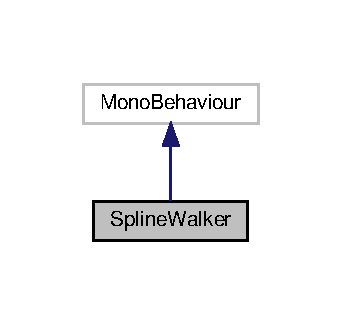
\includegraphics[width=164pt]{classSplineWalker__inherit__graph}
\end{center}
\end{figure}


Collaboration diagram for Spline\+Walker\+:\nopagebreak
\begin{figure}[H]
\begin{center}
\leavevmode
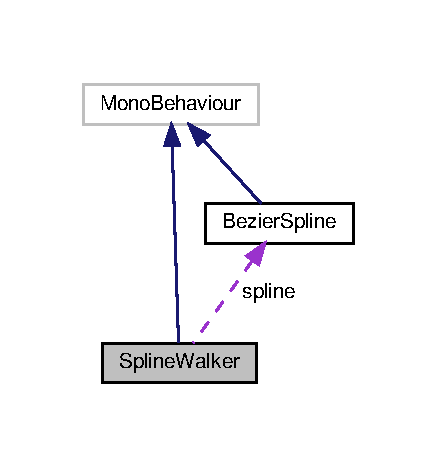
\includegraphics[width=210pt]{classSplineWalker__coll__graph}
\end{center}
\end{figure}
\subsection*{Public Attributes}
\begin{DoxyCompactItemize}
\item 
\hyperlink{classBezierSpline}{Bezier\+Spline} \hyperlink{classSplineWalker_ad55573118c9baae295b8bb272f03cc98}{spline}
\begin{DoxyCompactList}\small\item\em The Spline to follow\end{DoxyCompactList}\item 
bool \hyperlink{classSplineWalker_a7362491b40105af4e4f55c325257d7f7}{is\+Following} = false
\begin{DoxyCompactList}\small\item\em Is the Game\+Object following another one.\end{DoxyCompactList}\item 
bool \hyperlink{classSplineWalker_a21421e86b8ad0d38e04eadb1fcb0d57c}{is\+Driving}
\begin{DoxyCompactList}\small\item\em Is the Game\+Object using a realistic method to move.\end{DoxyCompactList}\item 
float \hyperlink{classSplineWalker_a26faffe76aa7172af19af857dc183d60}{velocity}
\begin{DoxyCompactList}\small\item\em Speed of the Game\+Object when controls are not handled by the driving car controller.\end{DoxyCompactList}\item 
Game\+Object \hyperlink{classSplineWalker_a98a7d49f715f41e9a7b5bfe779f11d75}{follows\+Game\+Object}
\begin{DoxyCompactList}\small\item\em If is\+Following is enabled, this is the Game\+Object to follow.\end{DoxyCompactList}\item 
float \hyperlink{classSplineWalker_a82080d499233b63d2cbde7274e2036b6}{distance\+Following} = 15f
\begin{DoxyCompactList}\small\item\em The wanted interdistance between the two Game\+Object. Only needed for the follower.\end{DoxyCompactList}\end{DoxyCompactItemize}
\subsection*{Properties}
\begin{DoxyCompactItemize}
\item 
float \hyperlink{classSplineWalker_a261aa79e4051461acff99d39f2b09a98}{progress}\hspace{0.3cm}{\ttfamily  \mbox{[}get, private set\mbox{]}}
\begin{DoxyCompactList}\small\item\em The progress of the Game\+Object over the Spline. Range from 0 to 1 in float.\end{DoxyCompactList}\end{DoxyCompactItemize}
\subsection*{Private Member Functions}
\begin{DoxyCompactItemize}
\item 
void \hyperlink{classSplineWalker_a7302455633490f68b15aad02b8fa54ca}{Start} ()
\begin{DoxyCompactList}\small\item\em Initialization of the class \end{DoxyCompactList}\item 
void \hyperlink{classSplineWalker_a9f250a7d108edae41325147ff1716db1}{Fixed\+Update} ()
\begin{DoxyCompactList}\small\item\em Updates the path every frame. \end{DoxyCompactList}\item 
float \hyperlink{classSplineWalker_a22d54e33aad18ea37775cea3229b7a72}{find\+Nearest\+Point\+In\+Spline} ()
\begin{DoxyCompactList}\small\item\em Find the nearest progress point from the leader Game\+Object in the spline. \end{DoxyCompactList}\item 
void \hyperlink{classSplineWalker_af1b6b1a3ede935316f1b5f686a2a9989}{look\+Forward} (float looking\+Distance)
\begin{DoxyCompactList}\small\item\em Force the Game\+Object to look forward the Spline. \end{DoxyCompactList}\end{DoxyCompactItemize}
\subsection*{Private Attributes}
\begin{DoxyCompactItemize}
\item 
Car\+Controller \hyperlink{classSplineWalker_ab8305528947e2a3ddfdbdc7b235640ab}{m\+\_\+\+Car}
\begin{DoxyCompactList}\small\item\em The realistic controller.\end{DoxyCompactList}\item 
const float \hyperlink{classSplineWalker_ae63367c40ff2c2c8ca29e43e42951a06}{sampling} = 100
\begin{DoxyCompactList}\small\item\em Discretisation of intervals.\end{DoxyCompactList}\end{DoxyCompactItemize}


\subsection{Detailed Description}
Class that handles the movements a Vehicle on a Spline. 

\href{https://catlikecoding.com/unity/tutorials/curves-and-splines/}{\tt https\+://catlikecoding.\+com/unity/tutorials/curves-\/and-\/splines/}

\subsection{Member Function Documentation}
\mbox{\Hypertarget{classSplineWalker_a22d54e33aad18ea37775cea3229b7a72}\label{classSplineWalker_a22d54e33aad18ea37775cea3229b7a72}} 
\index{Spline\+Walker@{Spline\+Walker}!find\+Nearest\+Point\+In\+Spline@{find\+Nearest\+Point\+In\+Spline}}
\index{find\+Nearest\+Point\+In\+Spline@{find\+Nearest\+Point\+In\+Spline}!Spline\+Walker@{Spline\+Walker}}
\subsubsection{\texorpdfstring{find\+Nearest\+Point\+In\+Spline()}{findNearestPointInSpline()}}
{\footnotesize\ttfamily float Spline\+Walker.\+find\+Nearest\+Point\+In\+Spline (\begin{DoxyParamCaption}{ }\end{DoxyParamCaption})\hspace{0.3cm}{\ttfamily [inline]}, {\ttfamily [private]}}



Find the nearest progress point from the leader Game\+Object in the spline. 

\begin{DoxyReturn}{Returns}
The value of progress.
\end{DoxyReturn}
\mbox{\Hypertarget{classSplineWalker_a9f250a7d108edae41325147ff1716db1}\label{classSplineWalker_a9f250a7d108edae41325147ff1716db1}} 
\index{Spline\+Walker@{Spline\+Walker}!Fixed\+Update@{Fixed\+Update}}
\index{Fixed\+Update@{Fixed\+Update}!Spline\+Walker@{Spline\+Walker}}
\subsubsection{\texorpdfstring{Fixed\+Update()}{FixedUpdate()}}
{\footnotesize\ttfamily void Spline\+Walker.\+Fixed\+Update (\begin{DoxyParamCaption}{ }\end{DoxyParamCaption})\hspace{0.3cm}{\ttfamily [inline]}, {\ttfamily [private]}}



Updates the path every frame. 

\mbox{\Hypertarget{classSplineWalker_af1b6b1a3ede935316f1b5f686a2a9989}\label{classSplineWalker_af1b6b1a3ede935316f1b5f686a2a9989}} 
\index{Spline\+Walker@{Spline\+Walker}!look\+Forward@{look\+Forward}}
\index{look\+Forward@{look\+Forward}!Spline\+Walker@{Spline\+Walker}}
\subsubsection{\texorpdfstring{look\+Forward()}{lookForward()}}
{\footnotesize\ttfamily void Spline\+Walker.\+look\+Forward (\begin{DoxyParamCaption}\item[{float}]{looking\+Distance }\end{DoxyParamCaption})\hspace{0.3cm}{\ttfamily [inline]}, {\ttfamily [private]}}



Force the Game\+Object to look forward the Spline. 


\begin{DoxyParams}{Parameters}
{\em looking\+Distance} & The distance the Game\+Object will look next on the spline. Can\textquotesingle{}t be higher than the two extremities distance.\\
\hline
\end{DoxyParams}
\begin{DoxyReturn}{Returns}
The value of progress.
\end{DoxyReturn}
\mbox{\Hypertarget{classSplineWalker_a7302455633490f68b15aad02b8fa54ca}\label{classSplineWalker_a7302455633490f68b15aad02b8fa54ca}} 
\index{Spline\+Walker@{Spline\+Walker}!Start@{Start}}
\index{Start@{Start}!Spline\+Walker@{Spline\+Walker}}
\subsubsection{\texorpdfstring{Start()}{Start()}}
{\footnotesize\ttfamily void Spline\+Walker.\+Start (\begin{DoxyParamCaption}{ }\end{DoxyParamCaption})\hspace{0.3cm}{\ttfamily [inline]}, {\ttfamily [private]}}



Initialization of the class 



\subsection{Member Data Documentation}
\mbox{\Hypertarget{classSplineWalker_a82080d499233b63d2cbde7274e2036b6}\label{classSplineWalker_a82080d499233b63d2cbde7274e2036b6}} 
\index{Spline\+Walker@{Spline\+Walker}!distance\+Following@{distance\+Following}}
\index{distance\+Following@{distance\+Following}!Spline\+Walker@{Spline\+Walker}}
\subsubsection{\texorpdfstring{distance\+Following}{distanceFollowing}}
{\footnotesize\ttfamily float Spline\+Walker.\+distance\+Following = 15f}



The wanted interdistance between the two Game\+Object. Only needed for the follower.

\mbox{\Hypertarget{classSplineWalker_a98a7d49f715f41e9a7b5bfe779f11d75}\label{classSplineWalker_a98a7d49f715f41e9a7b5bfe779f11d75}} 
\index{Spline\+Walker@{Spline\+Walker}!follows\+Game\+Object@{follows\+Game\+Object}}
\index{follows\+Game\+Object@{follows\+Game\+Object}!Spline\+Walker@{Spline\+Walker}}
\subsubsection{\texorpdfstring{follows\+Game\+Object}{followsGameObject}}
{\footnotesize\ttfamily Game\+Object Spline\+Walker.\+follows\+Game\+Object}



If is\+Following is enabled, this is the Game\+Object to follow.

\mbox{\Hypertarget{classSplineWalker_a21421e86b8ad0d38e04eadb1fcb0d57c}\label{classSplineWalker_a21421e86b8ad0d38e04eadb1fcb0d57c}} 
\index{Spline\+Walker@{Spline\+Walker}!is\+Driving@{is\+Driving}}
\index{is\+Driving@{is\+Driving}!Spline\+Walker@{Spline\+Walker}}
\subsubsection{\texorpdfstring{is\+Driving}{isDriving}}
{\footnotesize\ttfamily bool Spline\+Walker.\+is\+Driving}



Is the Game\+Object using a realistic method to move.

\mbox{\Hypertarget{classSplineWalker_a7362491b40105af4e4f55c325257d7f7}\label{classSplineWalker_a7362491b40105af4e4f55c325257d7f7}} 
\index{Spline\+Walker@{Spline\+Walker}!is\+Following@{is\+Following}}
\index{is\+Following@{is\+Following}!Spline\+Walker@{Spline\+Walker}}
\subsubsection{\texorpdfstring{is\+Following}{isFollowing}}
{\footnotesize\ttfamily bool Spline\+Walker.\+is\+Following = false}



Is the Game\+Object following another one.

\mbox{\Hypertarget{classSplineWalker_ab8305528947e2a3ddfdbdc7b235640ab}\label{classSplineWalker_ab8305528947e2a3ddfdbdc7b235640ab}} 
\index{Spline\+Walker@{Spline\+Walker}!m\+\_\+\+Car@{m\+\_\+\+Car}}
\index{m\+\_\+\+Car@{m\+\_\+\+Car}!Spline\+Walker@{Spline\+Walker}}
\subsubsection{\texorpdfstring{m\+\_\+\+Car}{m\_Car}}
{\footnotesize\ttfamily Car\+Controller Spline\+Walker.\+m\+\_\+\+Car\hspace{0.3cm}{\ttfamily [private]}}



The realistic controller.

\mbox{\Hypertarget{classSplineWalker_ae63367c40ff2c2c8ca29e43e42951a06}\label{classSplineWalker_ae63367c40ff2c2c8ca29e43e42951a06}} 
\index{Spline\+Walker@{Spline\+Walker}!sampling@{sampling}}
\index{sampling@{sampling}!Spline\+Walker@{Spline\+Walker}}
\subsubsection{\texorpdfstring{sampling}{sampling}}
{\footnotesize\ttfamily const float Spline\+Walker.\+sampling = 100\hspace{0.3cm}{\ttfamily [private]}}



Discretisation of intervals.

\mbox{\Hypertarget{classSplineWalker_ad55573118c9baae295b8bb272f03cc98}\label{classSplineWalker_ad55573118c9baae295b8bb272f03cc98}} 
\index{Spline\+Walker@{Spline\+Walker}!spline@{spline}}
\index{spline@{spline}!Spline\+Walker@{Spline\+Walker}}
\subsubsection{\texorpdfstring{spline}{spline}}
{\footnotesize\ttfamily \hyperlink{classBezierSpline}{Bezier\+Spline} Spline\+Walker.\+spline}



The Spline to follow

\mbox{\Hypertarget{classSplineWalker_a26faffe76aa7172af19af857dc183d60}\label{classSplineWalker_a26faffe76aa7172af19af857dc183d60}} 
\index{Spline\+Walker@{Spline\+Walker}!velocity@{velocity}}
\index{velocity@{velocity}!Spline\+Walker@{Spline\+Walker}}
\subsubsection{\texorpdfstring{velocity}{velocity}}
{\footnotesize\ttfamily float Spline\+Walker.\+velocity}



Speed of the Game\+Object when controls are not handled by the driving car controller.



\subsection{Property Documentation}
\mbox{\Hypertarget{classSplineWalker_a261aa79e4051461acff99d39f2b09a98}\label{classSplineWalker_a261aa79e4051461acff99d39f2b09a98}} 
\index{Spline\+Walker@{Spline\+Walker}!progress@{progress}}
\index{progress@{progress}!Spline\+Walker@{Spline\+Walker}}
\subsubsection{\texorpdfstring{progress}{progress}}
{\footnotesize\ttfamily float Spline\+Walker.\+progress\hspace{0.3cm}{\ttfamily [get]}, {\ttfamily [private set]}}



The progress of the Game\+Object over the Spline. Range from 0 to 1 in float.



The documentation for this class was generated from the following file\+:\begin{DoxyCompactItemize}
\item 
/root/\+Documents/\+Unity\+\_\+\+S\+T40/\+Suratram\+\_\+mixed\+Reality\+Simulator/\+Assets/\+Scripts/\+Bezier/\hyperlink{SplineWalker_8cs}{Spline\+Walker.\+cs}\end{DoxyCompactItemize}

\hypertarget{classSplineWalkerInspector}{}\section{Spline\+Walker\+Inspector Class Reference}
\label{classSplineWalkerInspector}\index{Spline\+Walker\+Inspector@{Spline\+Walker\+Inspector}}


Class that format the \hyperlink{classSplineWalker}{Spline\+Walker} settings to a more user-\/friendly one.  




Inheritance diagram for Spline\+Walker\+Inspector\+:\nopagebreak
\begin{figure}[H]
\begin{center}
\leavevmode
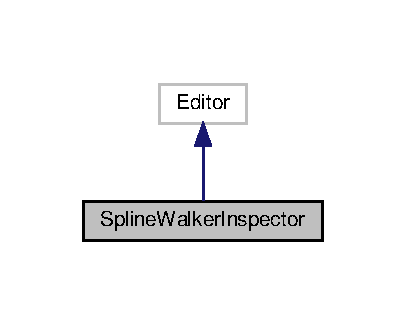
\includegraphics[width=195pt]{classSplineWalkerInspector__inherit__graph}
\end{center}
\end{figure}


Collaboration diagram for Spline\+Walker\+Inspector\+:\nopagebreak
\begin{figure}[H]
\begin{center}
\leavevmode
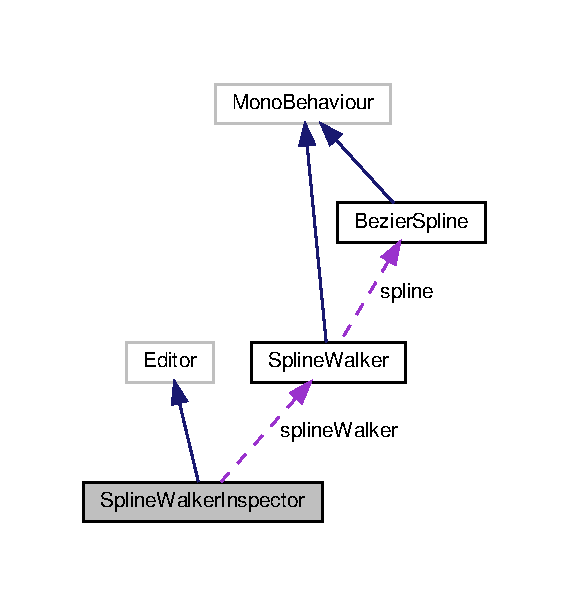
\includegraphics[width=273pt]{classSplineWalkerInspector__coll__graph}
\end{center}
\end{figure}
\subsection*{Public Member Functions}
\begin{DoxyCompactItemize}
\item 
override void \hyperlink{classSplineWalkerInspector_adaf5518940555970bf4d3c49624afb30}{On\+Inspector\+G\+UI} ()
\begin{DoxyCompactList}\small\item\em Updates the G\+UI \end{DoxyCompactList}\end{DoxyCompactItemize}
\subsection*{Private Attributes}
\begin{DoxyCompactItemize}
\item 
\hyperlink{classSplineWalker}{Spline\+Walker} \hyperlink{classSplineWalkerInspector_a97a8fd319093217c295ec9c45f5f1673}{spline\+Walker}
\begin{DoxyCompactList}\small\item\em The \hyperlink{classSplineWalker}{Spline\+Walker} that will be modified with the G\+UI.\end{DoxyCompactList}\end{DoxyCompactItemize}


\subsection{Detailed Description}
Class that format the \hyperlink{classSplineWalker}{Spline\+Walker} settings to a more user-\/friendly one. 



\subsection{Member Function Documentation}
\mbox{\Hypertarget{classSplineWalkerInspector_adaf5518940555970bf4d3c49624afb30}\label{classSplineWalkerInspector_adaf5518940555970bf4d3c49624afb30}} 
\index{Spline\+Walker\+Inspector@{Spline\+Walker\+Inspector}!On\+Inspector\+G\+UI@{On\+Inspector\+G\+UI}}
\index{On\+Inspector\+G\+UI@{On\+Inspector\+G\+UI}!Spline\+Walker\+Inspector@{Spline\+Walker\+Inspector}}
\subsubsection{\texorpdfstring{On\+Inspector\+G\+U\+I()}{OnInspectorGUI()}}
{\footnotesize\ttfamily override void Spline\+Walker\+Inspector.\+On\+Inspector\+G\+UI (\begin{DoxyParamCaption}{ }\end{DoxyParamCaption})\hspace{0.3cm}{\ttfamily [inline]}}



Updates the G\+UI 



\subsection{Member Data Documentation}
\mbox{\Hypertarget{classSplineWalkerInspector_a97a8fd319093217c295ec9c45f5f1673}\label{classSplineWalkerInspector_a97a8fd319093217c295ec9c45f5f1673}} 
\index{Spline\+Walker\+Inspector@{Spline\+Walker\+Inspector}!spline\+Walker@{spline\+Walker}}
\index{spline\+Walker@{spline\+Walker}!Spline\+Walker\+Inspector@{Spline\+Walker\+Inspector}}
\subsubsection{\texorpdfstring{spline\+Walker}{splineWalker}}
{\footnotesize\ttfamily \hyperlink{classSplineWalker}{Spline\+Walker} Spline\+Walker\+Inspector.\+spline\+Walker\hspace{0.3cm}{\ttfamily [private]}}



The \hyperlink{classSplineWalker}{Spline\+Walker} that will be modified with the G\+UI.



The documentation for this class was generated from the following file\+:\begin{DoxyCompactItemize}
\item 
/root/\+Documents/\+Unity\+\_\+\+S\+T40/\+Suratram\+\_\+mixed\+Reality\+Simulator/\+Assets/\+Scripts/\+Bezier/\+Editor/\hyperlink{SplineWalkerInspector_8cs}{Spline\+Walker\+Inspector.\+cs}\end{DoxyCompactItemize}

\chapter{File Documentation}
\hypertarget{Bezier_8cs}{}\section{/root/\+Documents/\+Unity\+\_\+\+S\+T40/\+Suratram\+\_\+mixed\+Reality\+Simulator/\+Assets/\+Scripts/\+Bezier/\+Bezier.cs File Reference}
\label{Bezier_8cs}\index{/root/\+Documents/\+Unity\+\_\+\+S\+T40/\+Suratram\+\_\+mixed\+Reality\+Simulator/\+Assets/\+Scripts/\+Bezier/\+Bezier.\+cs@{/root/\+Documents/\+Unity\+\_\+\+S\+T40/\+Suratram\+\_\+mixed\+Reality\+Simulator/\+Assets/\+Scripts/\+Bezier/\+Bezier.\+cs}}
\subsection*{Classes}
\begin{DoxyCompactItemize}
\item 
class {\bfseries Bezier}
\end{DoxyCompactItemize}

\hypertarget{BezierControlPointMode_8cs}{}\section{/root/\+Documents/\+Unity\+\_\+\+S\+T40/\+Suratram\+\_\+mixed\+Reality\+Simulator/\+Assets/\+Scripts/\+Bezier/\+Bezier\+Control\+Point\+Mode.cs File Reference}
\label{BezierControlPointMode_8cs}\index{/root/\+Documents/\+Unity\+\_\+\+S\+T40/\+Suratram\+\_\+mixed\+Reality\+Simulator/\+Assets/\+Scripts/\+Bezier/\+Bezier\+Control\+Point\+Mode.\+cs@{/root/\+Documents/\+Unity\+\_\+\+S\+T40/\+Suratram\+\_\+mixed\+Reality\+Simulator/\+Assets/\+Scripts/\+Bezier/\+Bezier\+Control\+Point\+Mode.\+cs}}
\subsection*{Enumerations}
\begin{DoxyCompactItemize}
\item 
enum \hyperlink{BezierControlPointMode_8cs_a41ff1a7271616f36cab397d937ee41b0}{Bezier\+Control\+Point\+Mode} \{ \hyperlink{BezierControlPointMode_8cs_a41ff1a7271616f36cab397d937ee41b0ab24ce0cd392a5b0b8dedc66c25213594}{Bezier\+Control\+Point\+Mode.\+Free}, 
\hyperlink{BezierControlPointMode_8cs_a41ff1a7271616f36cab397d937ee41b0a1d5b772bea21e5e949413e09eedf17de}{Bezier\+Control\+Point\+Mode.\+Aligned}, 
\hyperlink{BezierControlPointMode_8cs_a41ff1a7271616f36cab397d937ee41b0a3db6ae5ba47a2ce45b4788135adc8dcf}{Bezier\+Control\+Point\+Mode.\+Mirrored}
 \}
\end{DoxyCompactItemize}


\subsection{Enumeration Type Documentation}
\mbox{\Hypertarget{BezierControlPointMode_8cs_a41ff1a7271616f36cab397d937ee41b0}\label{BezierControlPointMode_8cs_a41ff1a7271616f36cab397d937ee41b0}} 
\index{Bezier\+Control\+Point\+Mode.\+cs@{Bezier\+Control\+Point\+Mode.\+cs}!Bezier\+Control\+Point\+Mode@{Bezier\+Control\+Point\+Mode}}
\index{Bezier\+Control\+Point\+Mode@{Bezier\+Control\+Point\+Mode}!Bezier\+Control\+Point\+Mode.\+cs@{Bezier\+Control\+Point\+Mode.\+cs}}
\subsubsection{\texorpdfstring{Bezier\+Control\+Point\+Mode}{BezierControlPointMode}}
{\footnotesize\ttfamily enum \hyperlink{BezierControlPointMode_8cs_a41ff1a7271616f36cab397d937ee41b0}{Bezier\+Control\+Point\+Mode}\hspace{0.3cm}{\ttfamily [strong]}}

\begin{DoxyEnumFields}{Enumerator}
\raisebox{\heightof{T}}[0pt][0pt]{\index{Free@{Free}!Bezier\+Control\+Point\+Mode.\+cs@{Bezier\+Control\+Point\+Mode.\+cs}}\index{Bezier\+Control\+Point\+Mode.\+cs@{Bezier\+Control\+Point\+Mode.\+cs}!Free@{Free}}}\mbox{\Hypertarget{BezierControlPointMode_8cs_a41ff1a7271616f36cab397d937ee41b0ab24ce0cd392a5b0b8dedc66c25213594}\label{BezierControlPointMode_8cs_a41ff1a7271616f36cab397d937ee41b0ab24ce0cd392a5b0b8dedc66c25213594}} 
Free&\\
\hline

\raisebox{\heightof{T}}[0pt][0pt]{\index{Aligned@{Aligned}!Bezier\+Control\+Point\+Mode.\+cs@{Bezier\+Control\+Point\+Mode.\+cs}}\index{Bezier\+Control\+Point\+Mode.\+cs@{Bezier\+Control\+Point\+Mode.\+cs}!Aligned@{Aligned}}}\mbox{\Hypertarget{BezierControlPointMode_8cs_a41ff1a7271616f36cab397d937ee41b0a1d5b772bea21e5e949413e09eedf17de}\label{BezierControlPointMode_8cs_a41ff1a7271616f36cab397d937ee41b0a1d5b772bea21e5e949413e09eedf17de}} 
Aligned&\\
\hline

\raisebox{\heightof{T}}[0pt][0pt]{\index{Mirrored@{Mirrored}!Bezier\+Control\+Point\+Mode.\+cs@{Bezier\+Control\+Point\+Mode.\+cs}}\index{Bezier\+Control\+Point\+Mode.\+cs@{Bezier\+Control\+Point\+Mode.\+cs}!Mirrored@{Mirrored}}}\mbox{\Hypertarget{BezierControlPointMode_8cs_a41ff1a7271616f36cab397d937ee41b0a3db6ae5ba47a2ce45b4788135adc8dcf}\label{BezierControlPointMode_8cs_a41ff1a7271616f36cab397d937ee41b0a3db6ae5ba47a2ce45b4788135adc8dcf}} 
Mirrored&\\
\hline

\end{DoxyEnumFields}

\hypertarget{BezierCurve_8cs}{}\section{/root/\+Documents/\+Unity\+\_\+\+S\+T40/\+Suratram\+\_\+mixed\+Reality\+Simulator/\+Assets/\+Scripts/\+Bezier/\+Bezier\+Curve.cs File Reference}
\label{BezierCurve_8cs}\index{/root/\+Documents/\+Unity\+\_\+\+S\+T40/\+Suratram\+\_\+mixed\+Reality\+Simulator/\+Assets/\+Scripts/\+Bezier/\+Bezier\+Curve.\+cs@{/root/\+Documents/\+Unity\+\_\+\+S\+T40/\+Suratram\+\_\+mixed\+Reality\+Simulator/\+Assets/\+Scripts/\+Bezier/\+Bezier\+Curve.\+cs}}
\subsection*{Classes}
\begin{DoxyCompactItemize}
\item 
class \hyperlink{classBezierCurve}{Bezier\+Curve}
\end{DoxyCompactItemize}

\hypertarget{BezierSpline_8cs}{}\section{/root/\+Documents/\+Unity\+\_\+\+S\+T40/\+Suratram\+\_\+mixed\+Reality\+Simulator/\+Assets/\+Scripts/\+Bezier/\+Bezier\+Spline.cs File Reference}
\label{BezierSpline_8cs}\index{/root/\+Documents/\+Unity\+\_\+\+S\+T40/\+Suratram\+\_\+mixed\+Reality\+Simulator/\+Assets/\+Scripts/\+Bezier/\+Bezier\+Spline.\+cs@{/root/\+Documents/\+Unity\+\_\+\+S\+T40/\+Suratram\+\_\+mixed\+Reality\+Simulator/\+Assets/\+Scripts/\+Bezier/\+Bezier\+Spline.\+cs}}
\subsection*{Classes}
\begin{DoxyCompactItemize}
\item 
class \hyperlink{classBezierSpline}{Bezier\+Spline}
\end{DoxyCompactItemize}

\hypertarget{easySpline_8cs}{}\section{/root/\+Documents/\+Unity\+\_\+\+S\+T40/\+Suratram\+\_\+mixed\+Reality\+Simulator/\+Assets/\+Scripts/\+Bezier/easy\+Spline.cs File Reference}
\label{easySpline_8cs}\index{/root/\+Documents/\+Unity\+\_\+\+S\+T40/\+Suratram\+\_\+mixed\+Reality\+Simulator/\+Assets/\+Scripts/\+Bezier/easy\+Spline.\+cs@{/root/\+Documents/\+Unity\+\_\+\+S\+T40/\+Suratram\+\_\+mixed\+Reality\+Simulator/\+Assets/\+Scripts/\+Bezier/easy\+Spline.\+cs}}
\subsection*{Classes}
\begin{DoxyCompactItemize}
\item 
class \hyperlink{classeasySpline}{easy\+Spline}
\begin{DoxyCompactList}\small\item\em Interface to adapt the size of the Spline. \end{DoxyCompactList}\end{DoxyCompactItemize}

\hypertarget{BezierCurveInspector_8cs}{}\section{/root/\+Documents/\+Unity\+\_\+\+S\+T40/\+Suratram\+\_\+mixed\+Reality\+Simulator/\+Assets/\+Scripts/\+Bezier/\+Editor/\+Bezier\+Curve\+Inspector.cs File Reference}
\label{BezierCurveInspector_8cs}\index{/root/\+Documents/\+Unity\+\_\+\+S\+T40/\+Suratram\+\_\+mixed\+Reality\+Simulator/\+Assets/\+Scripts/\+Bezier/\+Editor/\+Bezier\+Curve\+Inspector.\+cs@{/root/\+Documents/\+Unity\+\_\+\+S\+T40/\+Suratram\+\_\+mixed\+Reality\+Simulator/\+Assets/\+Scripts/\+Bezier/\+Editor/\+Bezier\+Curve\+Inspector.\+cs}}
\subsection*{Classes}
\begin{DoxyCompactItemize}
\item 
class \hyperlink{classBezierCurveInspector}{Bezier\+Curve\+Inspector}
\end{DoxyCompactItemize}

\hypertarget{BezierSplineInspector_8cs}{}\section{/root/\+Documents/\+Unity\+\_\+\+S\+T40/\+Suratram\+\_\+mixed\+Reality\+Simulator/\+Assets/\+Scripts/\+Bezier/\+Editor/\+Bezier\+Spline\+Inspector.cs File Reference}
\label{BezierSplineInspector_8cs}\index{/root/\+Documents/\+Unity\+\_\+\+S\+T40/\+Suratram\+\_\+mixed\+Reality\+Simulator/\+Assets/\+Scripts/\+Bezier/\+Editor/\+Bezier\+Spline\+Inspector.\+cs@{/root/\+Documents/\+Unity\+\_\+\+S\+T40/\+Suratram\+\_\+mixed\+Reality\+Simulator/\+Assets/\+Scripts/\+Bezier/\+Editor/\+Bezier\+Spline\+Inspector.\+cs}}
\subsection*{Classes}
\begin{DoxyCompactItemize}
\item 
class \hyperlink{classBezierSplineInspector}{Bezier\+Spline\+Inspector}
\end{DoxyCompactItemize}

\hypertarget{LineInspector_8cs}{}\section{/root/\+Documents/\+Unity\+\_\+\+S\+T40/\+Suratram\+\_\+mixed\+Reality\+Simulator/\+Assets/\+Scripts/\+Bezier/\+Editor/\+Line\+Inspector.cs File Reference}
\label{LineInspector_8cs}\index{/root/\+Documents/\+Unity\+\_\+\+S\+T40/\+Suratram\+\_\+mixed\+Reality\+Simulator/\+Assets/\+Scripts/\+Bezier/\+Editor/\+Line\+Inspector.\+cs@{/root/\+Documents/\+Unity\+\_\+\+S\+T40/\+Suratram\+\_\+mixed\+Reality\+Simulator/\+Assets/\+Scripts/\+Bezier/\+Editor/\+Line\+Inspector.\+cs}}
\subsection*{Classes}
\begin{DoxyCompactItemize}
\item 
class \hyperlink{classLineInspector}{Line\+Inspector}
\end{DoxyCompactItemize}

\hypertarget{SplineWalkerInspector_8cs}{}\section{/root/\+Documents/\+Unity\+\_\+\+S\+T40/\+Suratram\+\_\+mixed\+Reality\+Simulator/\+Assets/\+Scripts/\+Bezier/\+Editor/\+Spline\+Walker\+Inspector.cs File Reference}
\label{SplineWalkerInspector_8cs}\index{/root/\+Documents/\+Unity\+\_\+\+S\+T40/\+Suratram\+\_\+mixed\+Reality\+Simulator/\+Assets/\+Scripts/\+Bezier/\+Editor/\+Spline\+Walker\+Inspector.\+cs@{/root/\+Documents/\+Unity\+\_\+\+S\+T40/\+Suratram\+\_\+mixed\+Reality\+Simulator/\+Assets/\+Scripts/\+Bezier/\+Editor/\+Spline\+Walker\+Inspector.\+cs}}
\subsection*{Classes}
\begin{DoxyCompactItemize}
\item 
class \hyperlink{classSplineWalkerInspector}{Spline\+Walker\+Inspector}
\begin{DoxyCompactList}\small\item\em Class that format the \hyperlink{classSplineWalker}{Spline\+Walker} settings to a more user-\/friendly one. \end{DoxyCompactList}\end{DoxyCompactItemize}

\hypertarget{Line_8cs}{}\section{/root/\+Documents/\+Unity\+\_\+\+S\+T40/\+Suratram\+\_\+mixed\+Reality\+Simulator/\+Assets/\+Scripts/\+Bezier/\+Line.cs File Reference}
\label{Line_8cs}\index{/root/\+Documents/\+Unity\+\_\+\+S\+T40/\+Suratram\+\_\+mixed\+Reality\+Simulator/\+Assets/\+Scripts/\+Bezier/\+Line.\+cs@{/root/\+Documents/\+Unity\+\_\+\+S\+T40/\+Suratram\+\_\+mixed\+Reality\+Simulator/\+Assets/\+Scripts/\+Bezier/\+Line.\+cs}}
\subsection*{Classes}
\begin{DoxyCompactItemize}
\item 
class \hyperlink{classLine}{Line}
\end{DoxyCompactItemize}

\hypertarget{SplineWalker_8cs}{}\section{/root/\+Documents/\+Unity\+\_\+\+S\+T40/\+Suratram\+\_\+mixed\+Reality\+Simulator/\+Assets/\+Scripts/\+Bezier/\+Spline\+Walker.cs File Reference}
\label{SplineWalker_8cs}\index{/root/\+Documents/\+Unity\+\_\+\+S\+T40/\+Suratram\+\_\+mixed\+Reality\+Simulator/\+Assets/\+Scripts/\+Bezier/\+Spline\+Walker.\+cs@{/root/\+Documents/\+Unity\+\_\+\+S\+T40/\+Suratram\+\_\+mixed\+Reality\+Simulator/\+Assets/\+Scripts/\+Bezier/\+Spline\+Walker.\+cs}}
\subsection*{Classes}
\begin{DoxyCompactItemize}
\item 
class \hyperlink{classSplineWalker}{Spline\+Walker}
\begin{DoxyCompactList}\small\item\em Class that handles the movements a Vehicle on a Spline. \end{DoxyCompactList}\end{DoxyCompactItemize}

\hypertarget{monitoring_8cs}{}\section{/root/\+Documents/\+Unity\+\_\+\+S\+T40/\+Suratram\+\_\+mixed\+Reality\+Simulator/\+Assets/\+Scripts/monitoring.cs File Reference}
\label{monitoring_8cs}\index{/root/\+Documents/\+Unity\+\_\+\+S\+T40/\+Suratram\+\_\+mixed\+Reality\+Simulator/\+Assets/\+Scripts/monitoring.\+cs@{/root/\+Documents/\+Unity\+\_\+\+S\+T40/\+Suratram\+\_\+mixed\+Reality\+Simulator/\+Assets/\+Scripts/monitoring.\+cs}}
\subsection*{Classes}
\begin{DoxyCompactItemize}
\item 
class \hyperlink{classmonitoring}{monitoring}
\begin{DoxyCompactList}\small\item\em This class monitors, by retrieving differents informations in the scene. \end{DoxyCompactList}\end{DoxyCompactItemize}

\hypertarget{informations_8cs}{}\section{/root/\+Documents/\+Unity\+\_\+\+S\+T40/\+Suratram\+\_\+mixed\+Reality\+Simulator/\+Assets/\+Scripts/\+U\+I/informations.cs File Reference}
\label{informations_8cs}\index{/root/\+Documents/\+Unity\+\_\+\+S\+T40/\+Suratram\+\_\+mixed\+Reality\+Simulator/\+Assets/\+Scripts/\+U\+I/informations.\+cs@{/root/\+Documents/\+Unity\+\_\+\+S\+T40/\+Suratram\+\_\+mixed\+Reality\+Simulator/\+Assets/\+Scripts/\+U\+I/informations.\+cs}}
\subsection*{Classes}
\begin{DoxyCompactItemize}
\item 
class \hyperlink{classinformations}{informations}
\begin{DoxyCompactList}\small\item\em Class that displays some general informations on a Text component. \end{DoxyCompactList}\end{DoxyCompactItemize}

\hypertarget{mainpage_8doc}{}\section{mainpage.\+doc File Reference}
\label{mainpage_8doc}\index{mainpage.\+doc@{mainpage.\+doc}}

%--- End generated contents ---

% Index
\backmatter
\newpage
\phantomsection
\clearemptydoublepage
\addcontentsline{toc}{chapter}{Index}
\printindex

\end{document}
